\documentclass[twoside]{book}

% Packages required by doxygen
\usepackage{calc}
\usepackage{doxygen}
\usepackage{graphicx}
\usepackage[utf8]{inputenc}
\usepackage{makeidx}
\usepackage{multicol}
\usepackage{multirow}
\usepackage{textcomp}
\usepackage[table]{xcolor}

% Font selection
\usepackage[T1]{fontenc}
\usepackage{mathptmx}
\usepackage[scaled=.90]{helvet}
\usepackage{courier}
\usepackage{amssymb}
\usepackage{sectsty}
\renewcommand{\familydefault}{\sfdefault}
\allsectionsfont{%
  \fontseries{bc}\selectfont%
  \color{darkgray}%
}
\renewcommand{\DoxyLabelFont}{%
  \fontseries{bc}\selectfont%
  \color{darkgray}%
}

% Page & text layout
\usepackage{geometry}
\geometry{%
  a4paper,%
  top=2.5cm,%
  bottom=2.5cm,%
  left=2.5cm,%
  right=2.5cm%
}
\tolerance=750
\hfuzz=15pt
\hbadness=750
\setlength{\emergencystretch}{15pt}
\setlength{\parindent}{0cm}
\setlength{\parskip}{0.2cm}
\makeatletter
\renewcommand{\paragraph}{%
  \@startsection{paragraph}{4}{0ex}{-1.0ex}{1.0ex}{%
    \normalfont\normalsize\bfseries\SS@parafont%
  }%
}
\renewcommand{\subparagraph}{%
  \@startsection{subparagraph}{5}{0ex}{-1.0ex}{1.0ex}{%
    \normalfont\normalsize\bfseries\SS@subparafont%
  }%
}
\makeatother

% Headers & footers
\usepackage{fancyhdr}
\pagestyle{fancyplain}
\fancyhead[LE]{\fancyplain{}{\bfseries\thepage}}
\fancyhead[CE]{\fancyplain{}{}}
\fancyhead[RE]{\fancyplain{}{\bfseries\leftmark}}
\fancyhead[LO]{\fancyplain{}{\bfseries\rightmark}}
\fancyhead[CO]{\fancyplain{}{}}
\fancyhead[RO]{\fancyplain{}{\bfseries\thepage}}
\fancyfoot[LE]{\fancyplain{}{}}
\fancyfoot[CE]{\fancyplain{}{}}
\fancyfoot[RE]{\fancyplain{}{\bfseries\scriptsize Generated on Tue Jul 26 2016 05\-:49\-:11 for Electric Tiger Control Code by Doxygen }}
\fancyfoot[LO]{\fancyplain{}{\bfseries\scriptsize Generated on Tue Jul 26 2016 05\-:49\-:11 for Electric Tiger Control Code by Doxygen }}
\fancyfoot[CO]{\fancyplain{}{}}
\fancyfoot[RO]{\fancyplain{}{}}
\renewcommand{\footrulewidth}{0.4pt}
\renewcommand{\chaptermark}[1]{%
  \markboth{#1}{}%
}
\renewcommand{\sectionmark}[1]{%
  \markright{\thesection\ #1}%
}

% Indices & bibliography
\usepackage{natbib}
\usepackage[titles]{tocloft}
\setcounter{tocdepth}{3}
\setcounter{secnumdepth}{5}
\makeindex

% Hyperlinks (required, but should be loaded last)
\usepackage{ifpdf}
\ifpdf
  \usepackage[pdftex,pagebackref=true]{hyperref}
\else
  \usepackage[ps2pdf,pagebackref=true]{hyperref}
\fi
\hypersetup{%
  colorlinks=true,%
  linkcolor=blue,%
  citecolor=blue,%
  unicode%
}

% Custom commands
\newcommand{\clearemptydoublepage}{%
  \newpage{\pagestyle{empty}\cleardoublepage}%
}


%===== C O N T E N T S =====

\begin{document}

% Titlepage & ToC
\hypersetup{pageanchor=false}
\pagenumbering{roman}
\begin{titlepage}
\vspace*{7cm}
\begin{center}%
{\Large Electric Tiger Control Code \\[1ex]\large 0.\-1 }\\
\vspace*{1cm}
{\large Generated by Doxygen 1.8.6}\\
\vspace*{0.5cm}
{\small Tue Jul 26 2016 05:49:11}\\
\end{center}
\end{titlepage}
\clearemptydoublepage
\tableofcontents
\clearemptydoublepage
\pagenumbering{arabic}
\hypersetup{pageanchor=true}

%--- Begin generated contents ---
\chapter{Namespace Index}
\section{Packages}
Here are the packages with brief descriptions (if available)\-:\begin{DoxyCompactList}
\item\contentsline{section}{\hyperlink{namespacebase__functions}{base\-\_\-functions} }{\pageref{namespacebase__functions}}{}
\end{DoxyCompactList}

\chapter{Hierarchical Index}
\section{Class Hierarchy}
This inheritance list is sorted roughly, but not completely, alphabetically\-:\begin{DoxyCompactList}
\item \contentsline{section}{modetrack.\-\_\-object}{\pageref{classmodetrack_1_1__object}}{}
\begin{DoxyCompactList}
\item \contentsline{section}{modetrack.\-Mode\-Track}{\pageref{classmodetrack_1_1_mode_track}}{}
\end{DoxyCompactList}
\item \contentsline{section}{color\-\_\-printer.\-Color\-Printer}{\pageref{classcolor__printer_1_1_color_printer}}{}
\item \contentsline{section}{config\-\_\-classes.\-Config\-Types}{\pageref{classconfig__classes_1_1_config_types}}{}
\begin{DoxyCompactList}
\item \contentsline{section}{config\-\_\-classes.\-Base\-Types}{\pageref{classconfig__classes_1_1_base_types}}{}
\item \contentsline{section}{mode\-\_\-tracking.\-Mode\-Track\-Body}{\pageref{classmode__tracking_1_1_mode_track_body}}{}
\begin{DoxyCompactList}
\item \contentsline{section}{mode\-\_\-tracking.\-Mode\-Track\-Program}{\pageref{classmode__tracking_1_1_mode_track_program}}{}
\end{DoxyCompactList}
\end{DoxyCompactList}
\item \contentsline{section}{data\-\_\-processors.\-Convertor}{\pageref{classdata__processors_1_1_convertor}}{}
\item \contentsline{section}{data\-\_\-processors.\-Lorentzian\-Fitter}{\pageref{classdata__processors_1_1_lorentzian_fitter}}{}
\item \contentsline{section}{Mode\-Track}{\pageref{class_mode_track}}{}
\item \contentsline{section}{data\-\_\-processors.\-Plotter}{\pageref{classdata__processors_1_1_plotter}}{}
\item \contentsline{section}{Py\-Heap\-Type\-Object}{\pageref{struct_py_heap_type_object}}{}
\item \contentsline{section}{Retrieve\-Val}{\pageref{struct_retrieve_val}}{}
\item \contentsline{section}{socket\-\_\-communicators.\-Socket\-Comm}{\pageref{classsocket__communicators_1_1_socket_comm}}{}
\begin{DoxyCompactList}
\item \contentsline{section}{socket\-\_\-communicators.\-Network\-Analyzer\-Comm}{\pageref{classsocket__communicators_1_1_network_analyzer_comm}}{}
\item \contentsline{section}{socket\-\_\-communicators.\-Signal\-Analyzer\-Comm}{\pageref{classsocket__communicators_1_1_signal_analyzer_comm}}{}
\item \contentsline{section}{socket\-\_\-communicators.\-Stepper\-Motor\-Comm}{\pageref{classsocket__communicators_1_1_stepper_motor_comm}}{}
\item \contentsline{section}{socket\-\_\-communicators.\-Switch\-Comm}{\pageref{classsocket__communicators_1_1_switch_comm}}{}
\end{DoxyCompactList}
\item \contentsline{section}{socket\-\_\-connect\-\_\-2.\-Socket\-Comm}{\pageref{classsocket__connect__2_1_1_socket_comm}}{}
\item \contentsline{section}{swig\-\_\-cast\-\_\-info}{\pageref{structswig__cast__info}}{}
\item \contentsline{section}{swig\-\_\-const\-\_\-info}{\pageref{structswig__const__info}}{}
\item \contentsline{section}{swig\-\_\-globalvar}{\pageref{structswig__globalvar}}{}
\item \contentsline{section}{swig\-\_\-module\-\_\-info}{\pageref{structswig__module__info}}{}
\item \contentsline{section}{swig\-\_\-type\-\_\-info}{\pageref{structswig__type__info}}{}
\item \contentsline{section}{swig\-\_\-varlinkobject}{\pageref{structswig__varlinkobject}}{}
\item \contentsline{section}{swig\-:\-:Swig\-Ptr\-\_\-\-Py\-Object}{\pageref{classswig_1_1_swig_ptr___py_object}}{}
\begin{DoxyCompactList}
\item \contentsline{section}{swig\-:\-:Swig\-Var\-\_\-\-Py\-Object}{\pageref{structswig_1_1_swig_var___py_object}}{}
\end{DoxyCompactList}
\item \contentsline{section}{Swig\-Py\-Client\-Data}{\pageref{struct_swig_py_client_data}}{}
\item \contentsline{section}{Swig\-Py\-Object}{\pageref{struct_swig_py_object}}{}
\item \contentsline{section}{Swig\-Py\-Packed}{\pageref{struct_swig_py_packed}}{}
\end{DoxyCompactList}

\chapter{Class Index}
\section{Class List}
Here are the classes, structs, unions and interfaces with brief descriptions\-:\begin{DoxyCompactList}
\item\contentsline{section}{\hyperlink{classmodetrack_1_1__object}{modetrack.\-\_\-object} }{\pageref{classmodetrack_1_1__object}}{}
\item\contentsline{section}{\hyperlink{classconfig__classes_1_1_base_types}{config\-\_\-classes.\-Base\-Types} }{\pageref{classconfig__classes_1_1_base_types}}{}
\item\contentsline{section}{\hyperlink{classcolor__printer_1_1_color_printer}{color\-\_\-printer.\-Color\-Printer} }{\pageref{classcolor__printer_1_1_color_printer}}{}
\item\contentsline{section}{\hyperlink{classconfig__classes_1_1_config_types}{config\-\_\-classes.\-Config\-Types} }{\pageref{classconfig__classes_1_1_config_types}}{}
\item\contentsline{section}{\hyperlink{classdata__processors_1_1_convertor}{data\-\_\-processors.\-Convertor} }{\pageref{classdata__processors_1_1_convertor}}{}
\item\contentsline{section}{\hyperlink{classdata__processors_1_1_lorentzian_fitter}{data\-\_\-processors.\-Lorentzian\-Fitter} }{\pageref{classdata__processors_1_1_lorentzian_fitter}}{}
\item\contentsline{section}{\hyperlink{class_mode_track}{Mode\-Track} \\*Base Class for mode tracking algorithims; designed to be wrapped with Swig and called from Python module }{\pageref{class_mode_track}}{}
\item\contentsline{section}{\hyperlink{classmodetrack_1_1_mode_track}{modetrack.\-Mode\-Track} }{\pageref{classmodetrack_1_1_mode_track}}{}
\item\contentsline{section}{\hyperlink{classmode__tracking_1_1_mode_track_body}{mode\-\_\-tracking.\-Mode\-Track\-Body} }{\pageref{classmode__tracking_1_1_mode_track_body}}{}
\item\contentsline{section}{\hyperlink{classmode__tracking_1_1_mode_track_program}{mode\-\_\-tracking.\-Mode\-Track\-Program} }{\pageref{classmode__tracking_1_1_mode_track_program}}{}
\item\contentsline{section}{\hyperlink{classsocket__communicators_1_1_network_analyzer_comm}{socket\-\_\-communicators.\-Network\-Analyzer\-Comm} }{\pageref{classsocket__communicators_1_1_network_analyzer_comm}}{}
\item\contentsline{section}{\hyperlink{classdata__processors_1_1_plotter}{data\-\_\-processors.\-Plotter} }{\pageref{classdata__processors_1_1_plotter}}{}
\item\contentsline{section}{\hyperlink{struct_py_heap_type_object}{Py\-Heap\-Type\-Object} }{\pageref{struct_py_heap_type_object}}{}
\item\contentsline{section}{\hyperlink{struct_retrieve_val}{Retrieve\-Val} }{\pageref{struct_retrieve_val}}{}
\item\contentsline{section}{\hyperlink{classsocket__communicators_1_1_signal_analyzer_comm}{socket\-\_\-communicators.\-Signal\-Analyzer\-Comm} }{\pageref{classsocket__communicators_1_1_signal_analyzer_comm}}{}
\item\contentsline{section}{\hyperlink{classsocket__communicators_1_1_socket_comm}{socket\-\_\-communicators.\-Socket\-Comm} }{\pageref{classsocket__communicators_1_1_socket_comm}}{}
\item\contentsline{section}{\hyperlink{classsocket__connect__2_1_1_socket_comm}{socket\-\_\-connect\-\_\-2.\-Socket\-Comm} }{\pageref{classsocket__connect__2_1_1_socket_comm}}{}
\item\contentsline{section}{\hyperlink{classsocket__communicators_1_1_stepper_motor_comm}{socket\-\_\-communicators.\-Stepper\-Motor\-Comm} }{\pageref{classsocket__communicators_1_1_stepper_motor_comm}}{}
\item\contentsline{section}{\hyperlink{structswig__cast__info}{swig\-\_\-cast\-\_\-info} }{\pageref{structswig__cast__info}}{}
\item\contentsline{section}{\hyperlink{structswig__const__info}{swig\-\_\-const\-\_\-info} }{\pageref{structswig__const__info}}{}
\item\contentsline{section}{\hyperlink{structswig__globalvar}{swig\-\_\-globalvar} }{\pageref{structswig__globalvar}}{}
\item\contentsline{section}{\hyperlink{structswig__module__info}{swig\-\_\-module\-\_\-info} }{\pageref{structswig__module__info}}{}
\item\contentsline{section}{\hyperlink{structswig__type__info}{swig\-\_\-type\-\_\-info} }{\pageref{structswig__type__info}}{}
\item\contentsline{section}{\hyperlink{structswig__varlinkobject}{swig\-\_\-varlinkobject} }{\pageref{structswig__varlinkobject}}{}
\item\contentsline{section}{\hyperlink{classswig_1_1_swig_ptr___py_object}{swig\-::\-Swig\-Ptr\-\_\-\-Py\-Object} }{\pageref{classswig_1_1_swig_ptr___py_object}}{}
\item\contentsline{section}{\hyperlink{struct_swig_py_client_data}{Swig\-Py\-Client\-Data} }{\pageref{struct_swig_py_client_data}}{}
\item\contentsline{section}{\hyperlink{struct_swig_py_object}{Swig\-Py\-Object} }{\pageref{struct_swig_py_object}}{}
\item\contentsline{section}{\hyperlink{struct_swig_py_packed}{Swig\-Py\-Packed} }{\pageref{struct_swig_py_packed}}{}
\item\contentsline{section}{\hyperlink{structswig_1_1_swig_var___py_object}{swig\-::\-Swig\-Var\-\_\-\-Py\-Object} }{\pageref{structswig_1_1_swig_var___py_object}}{}
\item\contentsline{section}{\hyperlink{classsocket__communicators_1_1_switch_comm}{socket\-\_\-communicators.\-Switch\-Comm} }{\pageref{classsocket__communicators_1_1_switch_comm}}{}
\end{DoxyCompactList}

\chapter{Namespace Documentation}
\hypertarget{namespacebase__functions}{\section{base\-\_\-functions Namespace Reference}
\label{namespacebase__functions}\index{base\-\_\-functions@{base\-\_\-functions}}
}
\subsection*{Functions}
\begin{DoxyCompactItemize}
\item 
def \hyperlink{namespacebase__functions_aafaf676e7d2e85407d93582876e0fc78}{lorentzian}
\item 
def \hyperlink{namespacebase__functions_ac6b43d21a149ec318825184dafa16779}{within\-\_\-bounds}
\item 
\hypertarget{namespacebase__functions_acb1468fbd4a1e4a2ea708bb8940f9b90}{def {\bfseries residuals}}\label{namespacebase__functions_acb1468fbd4a1e4a2ea708bb8940f9b90}

\item 
\hypertarget{namespacebase__functions_ab79c7376c5d0710cf90a08c5f5e0febb}{def {\bfseries fit\-\_\-lorentzian}}\label{namespacebase__functions_ab79c7376c5d0710cf90a08c5f5e0febb}

\item 
\hypertarget{namespacebase__functions_a4950a5e86cc36dcf02cc6e6ab8fcb92c}{def {\bfseries c\-\_\-print}}\label{namespacebase__functions_a4950a5e86cc36dcf02cc6e6ab8fcb92c}

\item 
\hypertarget{namespacebase__functions_ab9ae59e5aac4be2f2a16c39f75ca4b8d}{def {\bfseries set\-\_\-\-G\-P\-I\-B}}\label{namespacebase__functions_ab9ae59e5aac4be2f2a16c39f75ca4b8d}

\item 
\hypertarget{namespacebase__functions_a91c83d9ec0d481b7b90512002cb8f9fc}{def {\bfseries set\-\_\-network\-\_\-analyzer}}\label{namespacebase__functions_a91c83d9ec0d481b7b90512002cb8f9fc}

\item 
\hypertarget{namespacebase__functions_ac5f7330d31c470d70a3fc906b390e802}{def {\bfseries set\-\_\-\-R\-F\-\_\-mapping}}\label{namespacebase__functions_ac5f7330d31c470d70a3fc906b390e802}

\item 
\hypertarget{namespacebase__functions_ad99612eb3c0f5c0f3ae9134a0268ae19}{def {\bfseries collect\-\_\-data}}\label{namespacebase__functions_ad99612eb3c0f5c0f3ae9134a0268ae19}

\item 
def \hyperlink{namespacebase__functions_afe3cd8a6ce6202fa936af55e4e510810}{make\-\_\-plot\-\_\-points}
\item 
\hypertarget{namespacebase__functions_a069a8429036101edd117a2d861ef7d53}{def {\bfseries get\-\_\-step\-\_\-sock}}\label{namespacebase__functions_a069a8429036101edd117a2d861ef7d53}

\item 
\hypertarget{namespacebase__functions_a65a8d03ee33d569536ffdaf12f9dfcd6}{def {\bfseries set\-\_\-stepper\-\_\-motor}}\label{namespacebase__functions_a65a8d03ee33d569536ffdaf12f9dfcd6}

\item 
\hypertarget{namespacebase__functions_a964351e00fc94877f43166181f74321c}{def {\bfseries reset\-\_\-cavity}}\label{namespacebase__functions_a964351e00fc94877f43166181f74321c}

\item 
\hypertarget{namespacebase__functions_ab1488bb8beb29a963d8a1a9ad8f5ee03}{def {\bfseries walk\-\_\-loop}}\label{namespacebase__functions_ab1488bb8beb29a963d8a1a9ad8f5ee03}

\item 
\hypertarget{namespacebase__functions_a721545f51eb209d733c2d8769731f396}{def {\bfseries set\-\_\-freq\-\_\-window}}\label{namespacebase__functions_a721545f51eb209d733c2d8769731f396}

\item 
\hypertarget{namespacebase__functions_a97686f2216ab139b66b249c8e0e3c014}{def {\bfseries take\-\_\-data\-\_\-single}}\label{namespacebase__functions_a97686f2216ab139b66b249c8e0e3c014}

\item 
\hypertarget{namespacebase__functions_a89296f642786dc37ad7194a024c12a28}{def {\bfseries str\-\_\-list\-\_\-to\-\_\-power\-\_\-list}}\label{namespacebase__functions_a89296f642786dc37ad7194a024c12a28}

\item 
\hypertarget{namespacebase__functions_afaa5d13d3c87e878e56fcbe95ffe90af}{def {\bfseries str\-\_\-to\-\_\-power\-\_\-list}}\label{namespacebase__functions_afaa5d13d3c87e878e56fcbe95ffe90af}

\item 
\hypertarget{namespacebase__functions_acb9ee05d208d2ed8a176a0104af06a0f}{def {\bfseries plot\-\_\-freq\-\_\-window}}\label{namespacebase__functions_acb9ee05d208d2ed8a176a0104af06a0f}

\item 
\hypertarget{namespacebase__functions_a1d57fe88685d6cec9f19ac23d52752ba}{def {\bfseries power\-\_\-list\-\_\-to\-\_\-str}}\label{namespacebase__functions_a1d57fe88685d6cec9f19ac23d52752ba}

\end{DoxyCompactItemize}


\subsection{Detailed Description}
\begin{DoxyVerb}Modules of functions that are used by all three principal classes-
ModeTracking, ModeMap, and ReflectionMap.

Each class utilizes these functions but does -not- inherit from this
module directly.

Functions
\end{DoxyVerb}
 

\subsection{Function Documentation}
\hypertarget{namespacebase__functions_aafaf676e7d2e85407d93582876e0fc78}{\index{base\-\_\-functions@{base\-\_\-functions}!lorentzian@{lorentzian}}
\index{lorentzian@{lorentzian}!base_functions@{base\-\_\-functions}}
\subsubsection[{lorentzian}]{\setlength{\rightskip}{0pt plus 5cm}def base\-\_\-functions.\-lorentzian (
\begin{DoxyParamCaption}
\item[{}]{x, }
\item[{}]{p}
\end{DoxyParamCaption}
)}}\label{namespacebase__functions_aafaf676e7d2e85407d93582876e0fc78}
\begin{DoxyVerb}Calculate Lorentz Line Shape.

Used for determining Q of a particular peak.

Args:
    p:List of parameters of the form [HWHM, Center, Height]
\end{DoxyVerb}
 \hypertarget{namespacebase__functions_afe3cd8a6ce6202fa936af55e4e510810}{\index{base\-\_\-functions@{base\-\_\-functions}!make\-\_\-plot\-\_\-points@{make\-\_\-plot\-\_\-points}}
\index{make\-\_\-plot\-\_\-points@{make\-\_\-plot\-\_\-points}!base_functions@{base\-\_\-functions}}
\subsubsection[{make\-\_\-plot\-\_\-points}]{\setlength{\rightskip}{0pt plus 5cm}def base\-\_\-functions.\-make\-\_\-plot\-\_\-points (
\begin{DoxyParamCaption}
\item[{}]{cavity\-\_\-length, }
\item[{}]{nominal\-\_\-centers, }
\item[{}]{nwa\-\_\-span, }
\item[{}]{nwa\-\_\-points, }
\item[{}]{raw\-\_\-nwa\-\_\-data}
\end{DoxyParamCaption}
)}}\label{namespacebase__functions_afe3cd8a6ce6202fa936af55e4e510810}
\begin{DoxyVerb}Convert collected data into a format suitable for saving or processing.
Output data will be a list of triples (Frequency(mHz),Cavity Length(in),Power(dBm))

Args:
    config_pars:ConfigParameters class
    constants:Constants class
    rt_params:RunTimeParameters class

Returns:
    plot_points, a list of data triples with the format described above
\end{DoxyVerb}
 \hypertarget{namespacebase__functions_ac6b43d21a149ec318825184dafa16779}{\index{base\-\_\-functions@{base\-\_\-functions}!within\-\_\-bounds@{within\-\_\-bounds}}
\index{within\-\_\-bounds@{within\-\_\-bounds}!base_functions@{base\-\_\-functions}}
\subsubsection[{within\-\_\-bounds}]{\setlength{\rightskip}{0pt plus 5cm}def base\-\_\-functions.\-within\-\_\-bounds (
\begin{DoxyParamCaption}
\item[{}]{p, }
\item[{}]{center\-\_\-freq, }
\item[{}]{freq\-\_\-window}
\end{DoxyParamCaption}
)}}\label{namespacebase__functions_ac6b43d21a149ec318825184dafa16779}
\begin{DoxyVerb}Check whether values for Lorentzian best fit curve are within reasonable
bounds.

Args:
    p:List of parameters
    center_freq: Center of the frequency window where the Lorentzian will be fitted
    freq_window: Width of of the frequency window centered at center_freq
    class.

Returns:
    True if within reasonable bounds, False otherwise
\end{DoxyVerb}
 
\chapter{Class Documentation}
\hypertarget{classmodetrack_1_1__object}{\section{modetrack.\-\_\-object Class Reference}
\label{classmodetrack_1_1__object}\index{modetrack.\-\_\-object@{modetrack.\-\_\-object}}
}
Inheritance diagram for modetrack.\-\_\-object\-:\begin{figure}[H]
\begin{center}
\leavevmode
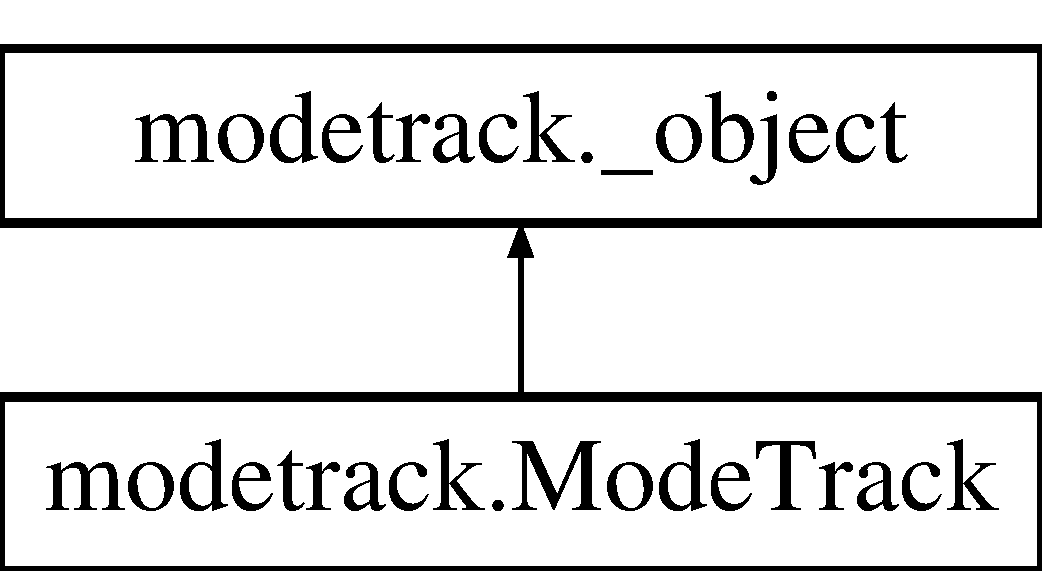
\includegraphics[height=2.000000cm]{classmodetrack_1_1__object}
\end{center}
\end{figure}


The documentation for this class was generated from the following file\-:\begin{DoxyCompactItemize}
\item 
/home/bephillips2/workspace/\-Electric\-\_\-\-Tiger\-\_\-\-Control\-\_\-\-Code/modetrack.\-py\end{DoxyCompactItemize}

\hypertarget{classconfig__classes_1_1_base_types}{\section{config\-\_\-classes.\-Base\-Types Class Reference}
\label{classconfig__classes_1_1_base_types}\index{config\-\_\-classes.\-Base\-Types@{config\-\_\-classes.\-Base\-Types}}
}
Inheritance diagram for config\-\_\-classes.\-Base\-Types\-:\begin{figure}[H]
\begin{center}
\leavevmode
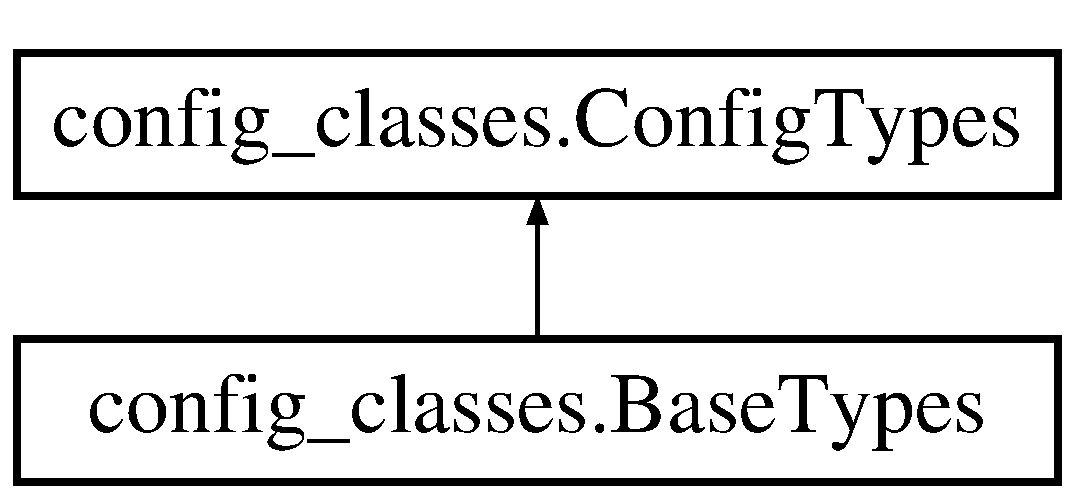
\includegraphics[height=2.000000cm]{classconfig__classes_1_1_base_types}
\end{center}
\end{figure}
\subsection*{Public Member Functions}
\begin{DoxyCompactItemize}
\item 
\hypertarget{classconfig__classes_1_1_base_types_a880a41ddba00206b3fa7d6c1aeee2e31}{def {\bfseries \-\_\-\-\_\-init\-\_\-\-\_\-}}\label{classconfig__classes_1_1_base_types_a880a41ddba00206b3fa7d6c1aeee2e31}

\item 
def \hyperlink{classconfig__classes_1_1_base_types_aead92a42a0e8ffd6d19a7ef43adb402d}{clear\-\_\-lists}
\end{DoxyCompactItemize}
\subsection*{Public Attributes}
\begin{DoxyCompactItemize}
\item 
\hypertarget{classconfig__classes_1_1_base_types_aa6645b65b8de1ff3ced95ffb9a8993d4}{{\bfseries actual\-\_\-center\-\_\-freq\-\_\-unrounded}}\label{classconfig__classes_1_1_base_types_aa6645b65b8de1ff3ced95ffb9a8993d4}

\item 
\hypertarget{classconfig__classes_1_1_base_types_a086191199277ecc77609e591937aa188}{{\bfseries actual\-\_\-center\-\_\-freq}}\label{classconfig__classes_1_1_base_types_a086191199277ecc77609e591937aa188}

\item 
\hypertarget{classconfig__classes_1_1_base_types_a61dc79c545bb18070b9ea008ae001771}{{\bfseries nwa\-\_\-fit\-\_\-data}}\label{classconfig__classes_1_1_base_types_a61dc79c545bb18070b9ea008ae001771}

\item 
\hypertarget{classconfig__classes_1_1_base_types_a025d74d4d7ad410391417d0f27fed170}{{\bfseries raw\-\_\-nwa\-\_\-data}}\label{classconfig__classes_1_1_base_types_a025d74d4d7ad410391417d0f27fed170}

\item 
\hypertarget{classconfig__classes_1_1_base_types_a7bcfb32fd583a5a312bc86834750fc3b}{{\bfseries background\-\_\-data}}\label{classconfig__classes_1_1_base_types_a7bcfb32fd583a5a312bc86834750fc3b}

\item 
\hypertarget{classconfig__classes_1_1_base_types_aa694d7969a718ca807d4b172af980208}{{\bfseries iterations}}\label{classconfig__classes_1_1_base_types_aa694d7969a718ca807d4b172af980208}

\item 
\hypertarget{classconfig__classes_1_1_base_types_a697c1aa3ec5ffe2f9590dc6d24e10e13}{{\bfseries number\-\_\-of\-\_\-iterations}}\label{classconfig__classes_1_1_base_types_a697c1aa3ec5ffe2f9590dc6d24e10e13}

\item 
\hypertarget{classconfig__classes_1_1_base_types_ad63e47ba6eb5215a564b538bbf45a7e9}{{\bfseries nsteps}}\label{classconfig__classes_1_1_base_types_ad63e47ba6eb5215a564b538bbf45a7e9}

\item 
\hypertarget{classconfig__classes_1_1_base_types_a2d63ea9d6aaeaf5dcf75a3a398798de0}{{\bfseries num\-\_\-of\-\_\-iters}}\label{classconfig__classes_1_1_base_types_a2d63ea9d6aaeaf5dcf75a3a398798de0}

\end{DoxyCompactItemize}


\subsection{Detailed Description}
\begin{DoxyVerb}Contains data that is mutable during run time, but does not need to be saved after program exits.
Class is designed to be accessed and have member variable values changed by external functions.
\end{DoxyVerb}
 

\subsection{Member Function Documentation}
\hypertarget{classconfig__classes_1_1_base_types_aead92a42a0e8ffd6d19a7ef43adb402d}{\index{config\-\_\-classes\-::\-Base\-Types@{config\-\_\-classes\-::\-Base\-Types}!clear\-\_\-lists@{clear\-\_\-lists}}
\index{clear\-\_\-lists@{clear\-\_\-lists}!config_classes::BaseTypes@{config\-\_\-classes\-::\-Base\-Types}}
\subsubsection[{clear\-\_\-lists}]{\setlength{\rightskip}{0pt plus 5cm}def config\-\_\-classes.\-Base\-Types.\-clear\-\_\-lists (
\begin{DoxyParamCaption}
\item[{}]{self}
\end{DoxyParamCaption}
)}}\label{classconfig__classes_1_1_base_types_aead92a42a0e8ffd6d19a7ef43adb402d}
\begin{DoxyVerb}Clear all raw data that was taken from the network analyzer
    needs to be called during loops so that data is not duplicated.
\end{DoxyVerb}
 

The documentation for this class was generated from the following file\-:\begin{DoxyCompactItemize}
\item 
/home/bephillips2/workspace/\-Electric\-\_\-\-Tiger\-\_\-\-Control\-\_\-\-Code/config\-\_\-classes.\-py\end{DoxyCompactItemize}

\hypertarget{classcolor__printer_1_1_color_printer}{\section{color\-\_\-printer.\-Color\-Printer Class Reference}
\label{classcolor__printer_1_1_color_printer}\index{color\-\_\-printer.\-Color\-Printer@{color\-\_\-printer.\-Color\-Printer}}
}
\subsection*{Public Member Functions}
\begin{DoxyCompactItemize}
\item 
\hypertarget{classcolor__printer_1_1_color_printer_a74f2b2ef4f1211d193bd5474098a7cee}{def {\bfseries \-\_\-\-\_\-init\-\_\-\-\_\-}}\label{classcolor__printer_1_1_color_printer_a74f2b2ef4f1211d193bd5474098a7cee}

\item 
\hypertarget{classcolor__printer_1_1_color_printer_acd3a518f898ebc3ad122b7d15d97f656}{def {\bfseries \-\_\-\-\_\-call\-\_\-\-\_\-}}\label{classcolor__printer_1_1_color_printer_acd3a518f898ebc3ad122b7d15d97f656}

\end{DoxyCompactItemize}
\subsection*{Public Attributes}
\begin{DoxyCompactItemize}
\item 
\hypertarget{classcolor__printer_1_1_color_printer_a263db729cb9e2df87bcbc8c3bc41e052}{{\bfseries head}}\label{classcolor__printer_1_1_color_printer_a263db729cb9e2df87bcbc8c3bc41e052}

\end{DoxyCompactItemize}


The documentation for this class was generated from the following file\-:\begin{DoxyCompactItemize}
\item 
/home/bephillips2/workspace/\-Electric\-\_\-\-Tiger\-\_\-\-Control\-\_\-\-Code/color\-\_\-printer.\-py\end{DoxyCompactItemize}

\hypertarget{classconfig__classes_1_1_config_types}{\section{config\-\_\-classes.\-Config\-Types Class Reference}
\label{classconfig__classes_1_1_config_types}\index{config\-\_\-classes.\-Config\-Types@{config\-\_\-classes.\-Config\-Types}}
}
Inheritance diagram for config\-\_\-classes.\-Config\-Types\-:\begin{figure}[H]
\begin{center}
\leavevmode
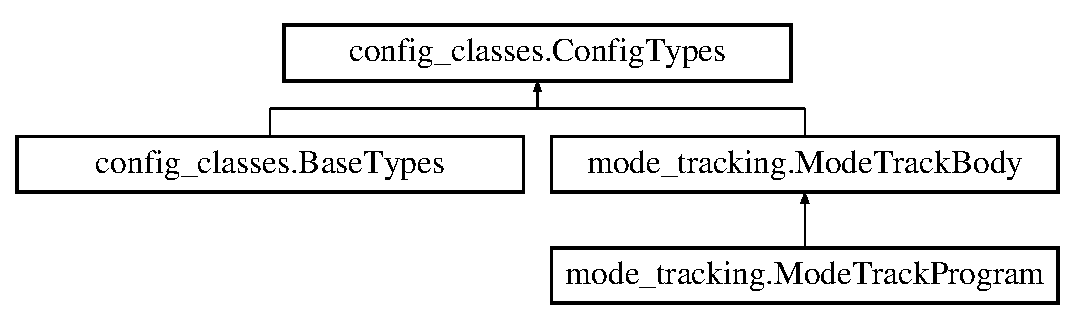
\includegraphics[height=3.000000cm]{classconfig__classes_1_1_config_types}
\end{center}
\end{figure}
\subsection*{Public Member Functions}
\begin{DoxyCompactItemize}
\item 
def \hyperlink{classconfig__classes_1_1_config_types_ae72c95b861cdf7720bac010da60bd082}{\-\_\-\-\_\-init\-\_\-\-\_\-}
\item 
def \hyperlink{classconfig__classes_1_1_config_types_a73e7c999dc01bc081ae866d485be3836}{close\-\_\-all}
\end{DoxyCompactItemize}
\subsection*{Public Attributes}
\begin{DoxyCompactItemize}
\item 
\hypertarget{classconfig__classes_1_1_config_types_a34ce9f770593d52d488c15078aaaf139}{{\bfseries print\-\_\-green}}\label{classconfig__classes_1_1_config_types_a34ce9f770593d52d488c15078aaaf139}

\item 
\hypertarget{classconfig__classes_1_1_config_types_a9751b795ba6bfef933f91cf3b6dd4505}{{\bfseries print\-\_\-purple}}\label{classconfig__classes_1_1_config_types_a9751b795ba6bfef933f91cf3b6dd4505}

\item 
\hypertarget{classconfig__classes_1_1_config_types_a064692a58bf56ea42d3ac3f5f4fa73b3}{{\bfseries print\-\_\-blue}}\label{classconfig__classes_1_1_config_types_a064692a58bf56ea42d3ac3f5f4fa73b3}

\item 
\hypertarget{classconfig__classes_1_1_config_types_acf58fae99cf73fb829bea02f4c37dccf}{{\bfseries print\-\_\-red}}\label{classconfig__classes_1_1_config_types_acf58fae99cf73fb829bea02f4c37dccf}

\item 
\hypertarget{classconfig__classes_1_1_config_types_a6d67331a2645674e277620507d715521}{{\bfseries sock\-\_\-dict}}\label{classconfig__classes_1_1_config_types_a6d67331a2645674e277620507d715521}

\item 
\hypertarget{classconfig__classes_1_1_config_types_ad8abbf130e01aef1a3df21e9610d796f}{{\bfseries data\-\_\-dict}}\label{classconfig__classes_1_1_config_types_ad8abbf130e01aef1a3df21e9610d796f}

\item 
\hypertarget{classconfig__classes_1_1_config_types_a66280f7aa817c2bfa3c80973041ae53c}{{\bfseries addr\-\_\-dict}}\label{classconfig__classes_1_1_config_types_a66280f7aa817c2bfa3c80973041ae53c}

\item 
\hypertarget{classconfig__classes_1_1_config_types_a941d66a12dd918e27fc2d0c2ae784194}{{\bfseries sock\-\_\-comm}}\label{classconfig__classes_1_1_config_types_a941d66a12dd918e27fc2d0c2ae784194}

\end{DoxyCompactItemize}


\subsection{Detailed Description}
\begin{DoxyVerb}Contains data that is read from user specified config file.
Class is responsible for reading and parsing config file, as well as generating
socket objects for all instruments.
Makes use of two dictionaries, data_dict for plain data types and sock_dict for socket objects.

Member variables in data_dict are mutable during run time, members of sock_dict are not.

Attributes:
    sock_data: Dictionary that holds socket objects, format is instrument_name:[socket_object]
    data_dict: Dictionary that hold plain data loaded from the config file, format is data_title:[data_value]
\end{DoxyVerb}
 

\subsection{Constructor \& Destructor Documentation}
\hypertarget{classconfig__classes_1_1_config_types_ae72c95b861cdf7720bac010da60bd082}{\index{config\-\_\-classes\-::\-Config\-Types@{config\-\_\-classes\-::\-Config\-Types}!\-\_\-\-\_\-init\-\_\-\-\_\-@{\-\_\-\-\_\-init\-\_\-\-\_\-}}
\index{\-\_\-\-\_\-init\-\_\-\-\_\-@{\-\_\-\-\_\-init\-\_\-\-\_\-}!config_classes::ConfigTypes@{config\-\_\-classes\-::\-Config\-Types}}
\subsubsection[{\-\_\-\-\_\-init\-\_\-\-\_\-}]{\setlength{\rightskip}{0pt plus 5cm}def config\-\_\-classes.\-Config\-Types.\-\_\-\-\_\-init\-\_\-\-\_\- (
\begin{DoxyParamCaption}
\item[{}]{self, }
\item[{}]{config\-\_\-path}
\end{DoxyParamCaption}
)}}\label{classconfig__classes_1_1_config_types_ae72c95b861cdf7720bac010da60bd082}
\begin{DoxyVerb}Initailzie dictionary objects, and populate from config file information.

Args:
    config_path: string specifying path to config file, set by command line argument.
\end{DoxyVerb}
 

\subsection{Member Function Documentation}
\hypertarget{classconfig__classes_1_1_config_types_a73e7c999dc01bc081ae866d485be3836}{\index{config\-\_\-classes\-::\-Config\-Types@{config\-\_\-classes\-::\-Config\-Types}!close\-\_\-all@{close\-\_\-all}}
\index{close\-\_\-all@{close\-\_\-all}!config_classes::ConfigTypes@{config\-\_\-classes\-::\-Config\-Types}}
\subsubsection[{close\-\_\-all}]{\setlength{\rightskip}{0pt plus 5cm}def config\-\_\-classes.\-Config\-Types.\-close\-\_\-all (
\begin{DoxyParamCaption}
\item[{}]{self}
\end{DoxyParamCaption}
)}}\label{classconfig__classes_1_1_config_types_a73e7c999dc01bc081ae866d485be3836}
\begin{DoxyVerb}Function to close all sockets in the socket dictionary, to be called before program exit or during error handling
    should not throw errors since sockets should only be added to dictionary when connection was successful, avoiding the case of a NULL value
\end{DoxyVerb}
 

The documentation for this class was generated from the following file\-:\begin{DoxyCompactItemize}
\item 
/home/bephillips2/workspace/\-Electric\-\_\-\-Tiger\-\_\-\-Control\-\_\-\-Code/config\-\_\-classes.\-py\end{DoxyCompactItemize}

\hypertarget{classdata__processors_1_1_convertor}{\section{data\-\_\-processors.\-Convertor Class Reference}
\label{classdata__processors_1_1_convertor}\index{data\-\_\-processors.\-Convertor@{data\-\_\-processors.\-Convertor}}
}
\subsection*{Public Member Functions}
\begin{DoxyCompactItemize}
\item 
\hypertarget{classdata__processors_1_1_convertor_a94e11e94ade77ad72d4e4d023743be0a}{def {\bfseries str\-\_\-list\-\_\-to\-\_\-power\-\_\-list}}\label{classdata__processors_1_1_convertor_a94e11e94ade77ad72d4e4d023743be0a}

\item 
\hypertarget{classdata__processors_1_1_convertor_a5e2186b5bf7c96c63dc2e2bdc732ea80}{def {\bfseries power\-\_\-list\-\_\-to\-\_\-str}}\label{classdata__processors_1_1_convertor_a5e2186b5bf7c96c63dc2e2bdc732ea80}

\item 
def \hyperlink{classdata__processors_1_1_convertor_a88faafccd5d1c63f535859ce1ce40b80}{make\-\_\-plot\-\_\-points}
\end{DoxyCompactItemize}


\subsection{Member Function Documentation}
\hypertarget{classdata__processors_1_1_convertor_a88faafccd5d1c63f535859ce1ce40b80}{\index{data\-\_\-processors\-::\-Convertor@{data\-\_\-processors\-::\-Convertor}!make\-\_\-plot\-\_\-points@{make\-\_\-plot\-\_\-points}}
\index{make\-\_\-plot\-\_\-points@{make\-\_\-plot\-\_\-points}!data_processors::Convertor@{data\-\_\-processors\-::\-Convertor}}
\subsubsection[{make\-\_\-plot\-\_\-points}]{\setlength{\rightskip}{0pt plus 5cm}def data\-\_\-processors.\-Convertor.\-make\-\_\-plot\-\_\-points (
\begin{DoxyParamCaption}
\item[{}]{self, }
\item[{}]{raw\-\_\-data, }
\item[{}]{cavity\-\_\-length, }
\item[{}]{min\-\_\-frequency, }
\item[{}]{max\-\_\-frequency}
\end{DoxyParamCaption}
)}}\label{classdata__processors_1_1_convertor_a88faafccd5d1c63f535859ce1ce40b80}
\begin{DoxyVerb}Convert collected data into a format suitable for saving or processing.
Output data will be a list of triples (Frequency(mHz),Cavity Length(in),Power(dBm))
    
Args:
    raw_data:Either a list of strings or a single string in comma seperated format
    cavity_length:The current length of the cavity in inches
    nominal_centers:RunTimeParameters class
    
Returns:
    plot_points, a list of data triples with the format described above
\end{DoxyVerb}
 

The documentation for this class was generated from the following file\-:\begin{DoxyCompactItemize}
\item 
/home/bephillips2/workspace/\-Electric\-\_\-\-Tiger\-\_\-\-Control\-\_\-\-Code/data\-\_\-processors.\-py\end{DoxyCompactItemize}

\hypertarget{classdata__processors_1_1_lorentzian_fitter}{\section{data\-\_\-processors.\-Lorentzian\-Fitter Class Reference}
\label{classdata__processors_1_1_lorentzian_fitter}\index{data\-\_\-processors.\-Lorentzian\-Fitter@{data\-\_\-processors.\-Lorentzian\-Fitter}}
}
\subsection*{Public Member Functions}
\begin{DoxyCompactItemize}
\item 
\hypertarget{classdata__processors_1_1_lorentzian_fitter_adc0517611d45e3fc0ffbaf3d65158fa5}{def {\bfseries \-\_\-\-\_\-init\-\_\-\-\_\-}}\label{classdata__processors_1_1_lorentzian_fitter_adc0517611d45e3fc0ffbaf3d65158fa5}

\item 
\hypertarget{classdata__processors_1_1_lorentzian_fitter_a2d7bcc2fd63903cc18d301a3c08c7ce6}{def {\bfseries \-\_\-\-\_\-call\-\_\-\-\_\-}}\label{classdata__processors_1_1_lorentzian_fitter_a2d7bcc2fd63903cc18d301a3c08c7ce6}

\end{DoxyCompactItemize}
\subsection*{Public Attributes}
\begin{DoxyCompactItemize}
\item 
\hypertarget{classdata__processors_1_1_lorentzian_fitter_ada40838b7c966657253b01b3c9520f59}{{\bfseries print\-\_\-yellow}}\label{classdata__processors_1_1_lorentzian_fitter_ada40838b7c966657253b01b3c9520f59}

\item 
\hypertarget{classdata__processors_1_1_lorentzian_fitter_a8af51db0e5453f33a165bf15ae19e0b9}{{\bfseries print\-\_\-purple}}\label{classdata__processors_1_1_lorentzian_fitter_a8af51db0e5453f33a165bf15ae19e0b9}

\end{DoxyCompactItemize}


The documentation for this class was generated from the following file\-:\begin{DoxyCompactItemize}
\item 
/home/bephillips2/workspace/\-Electric\-\_\-\-Tiger\-\_\-\-Control\-\_\-\-Code/data\-\_\-processors.\-py\end{DoxyCompactItemize}

\hypertarget{class_mode_track}{\section{Mode\-Track Class Reference}
\label{class_mode_track}\index{Mode\-Track@{Mode\-Track}}
}


Base Class for mode tracking algorithims; designed to be wrapped with Swig and called from Python module.  




{\ttfamily \#include $<$modetrack.\-h$>$}

\subsection*{Public Member Functions}
\begin{DoxyCompactItemize}
\item 
void \hyperlink{class_mode_track_a53130b8d183a69b14d2ef47666d09385}{From\-File} (std\-::string config\-\_\-name)
\begin{DoxyCompactList}\small\item\em Run mode tracking algorithim on previously saved data. \end{DoxyCompactList}\item 
void \hyperlink{class_mode_track_aa04491a2f3b4bb04fe6503757d416b73}{Set\-Background} (std\-::string background\-\_\-str)
\begin{DoxyCompactList}\small\item\em Set background data which will be subtracted from each measurement. \end{DoxyCompactList}\item 
double \hyperlink{class_mode_track_ac4ab8caa7ab71906390651cdd4c20c0c}{Get\-Peaks\-Gauss} (std\-::string data\-\_\-str, int mode\-\_\-number)
\begin{DoxyCompactList}\small\item\em Identify minima peaks in a list of power data using Gaussian filtering. \end{DoxyCompactList}\item 
double \hyperlink{class_mode_track_a2158f2117f99a3aee6891bcc2126aa83}{Get\-Peaks\-Bi\-Lat} (std\-::string data\-\_\-str, int mode\-\_\-number)
\begin{DoxyCompactList}\small\item\em Identify minima peaks in a list of power data using Bilateral filtering. \end{DoxyCompactList}\item 
double \hyperlink{class_mode_track_a8ffe12b39a5d90b6ba7a25c0c66bea8d}{Get\-Max\-Peak} (std\-::string data\-\_\-str)
\begin{DoxyCompactList}\small\item\em Find a local maximum in a list of data. \end{DoxyCompactList}\item 
\hypertarget{class_mode_track_a99eeeb6757873474994a61dbd7e31e43}{void {\bfseries Set\-Lower\-Bound} (double frequency)}\label{class_mode_track_a99eeeb6757873474994a61dbd7e31e43}

\item 
\hypertarget{class_mode_track_a7b7a1977d0cdacf2533581c82707e018}{void {\bfseries Set\-Upper\-Bound} (double frequency)}\label{class_mode_track_a7b7a1977d0cdacf2533581c82707e018}

\end{DoxyCompactItemize}
\subsection*{Protected Types}
\begin{DoxyCompactItemize}
\item 
enum {\bfseries Method} \{ {\bfseries Gauss}, 
{\bfseries Bi\-Lat}
 \}
\end{DoxyCompactItemize}
\subsection*{Protected Member Functions}
\begin{DoxyCompactItemize}
\item 
void \hyperlink{class_mode_track_a4e0a0d9430910d77c067c0ee40110200}{Load\-From\-Config} (const char $\ast$config\-\_\-name)
\begin{DoxyCompactList}\small\item\em opens file specified and loads values into enteries\-\_\-strings \end{DoxyCompactList}\item 
\hypertarget{class_mode_track_a992935ab5c2bd97e824a88039238e07f}{void \hyperlink{class_mode_track_a992935ab5c2bd97e824a88039238e07f}{Cast\-To\-Type} ()}\label{class_mode_track_a992935ab5c2bd97e824a88039238e07f}

\begin{DoxyCompactList}\small\item\em casts each element in enteries\-\_\-strings from a string to a double and loads into entries. \end{DoxyCompactList}\item 
std\-::vector$<$ double $>$ \hyperlink{class_mode_track_a8461b01cf1c811aa7cf781fb9bb07f68}{Derivative} (std\-::vector$<$ double $>$ \&data\-\_\-list)
\begin{DoxyCompactList}\small\item\em Compute the the forth order approximation of the derivative. \end{DoxyCompactList}\item 
void \hyperlink{class_mode_track_a5dccdca7cd909c332b5ed1e09118cd98}{Populate\-Best\-Fit\-Curves} ()
\begin{DoxyCompactList}\small\item\em Load cubic spline coeffecients for modes 0 through 3. \end{DoxyCompactList}\item 
double \hyperlink{class_mode_track_afe43b234695b74e5c493acb08aec39b7}{Std\-Dev} (std\-::vector$<$ double $>$ \&data\-\_\-list)
\begin{DoxyCompactList}\small\item\em Compute the standard deviation of a list. \end{DoxyCompactList}\item 
std\-::vector$<$ double $>$ \hyperlink{class_mode_track_ac9749deca774e487cbcc694a56b226cd}{Normalize} (std\-::vector$<$ double $>$ \&data\-\_\-list)
\begin{DoxyCompactList}\small\item\em Normalize a list of data w.\-r.\-t. to the L2 norm. \end{DoxyCompactList}\item 
std\-::vector$<$ double $>$ \hyperlink{class_mode_track_a8d08e12e9d882c875e6f7f4b8539f542}{Convolve} (std\-::vector$<$ double $>$ \&data\-\_\-list, std\-::vector$<$ double $>$ \&kernel)
\begin{DoxyCompactList}\small\item\em Compute the 1\-D convolution of data\-\_\-list with kernel. \end{DoxyCompactList}\item 
std\-::vector$<$ double $>$ \hyperlink{class_mode_track_aa315defc02162bed269fa981a01382b8}{Gauss\-Blur} (std\-::vector$<$ double $>$ \&data\-\_\-list)
\begin{DoxyCompactList}\small\item\em Compute the convulution of data\-\_\-list with a Gaussian kernel. \end{DoxyCompactList}\item 
std\-::vector$<$ double $>$ \hyperlink{class_mode_track_a69dab14db20b8ffdcae63914fb2e0c83}{Find\-Peaks} (std\-::vector$<$ double $>$ \&data\-\_\-list, Mode\-Track\-::\-Method method)
\begin{DoxyCompactList}\small\item\em Find minima peaks in a list. \end{DoxyCompactList}\item 
std\-::map$<$ uint, double $>$ \hyperlink{class_mode_track_a83776f06fac4ccff81ae76405dc5bee8}{Compare\-And\-Fill} (std\-::vector$<$ double $>$ \&peak\-\_\-list, std\-::vector$<$ std\-::tuple$<$ double, double, double $>$ $>$ \&comparison\-\_\-list)
\begin{DoxyCompactList}\small\item\em Compare the position of each identified peak with estimated peak position. \end{DoxyCompactList}\item 
double \hyperlink{class_mode_track_a7960f1ee58a1a420814843ca0f8c0ae4}{Generate\-Spline} (int mode\-\_\-number, double length)
\begin{DoxyCompactList}\small\item\em Generate\-Spline. \end{DoxyCompactList}\item 
std\-::vector$<$ double $>$ \hyperlink{class_mode_track_ad69c546f3d3ac916b0f00c7aa2917903}{Gauss\-Kernel} (int r)
\begin{DoxyCompactList}\small\item\em Generate a Gaussian kernel of radius r and sigma = r/2 Kernel is generated by sampling Gaussian function with sigma = r/2 a total of r times. \end{DoxyCompactList}\item 
void \hyperlink{class_mode_track_a9e59f0ed0b57daebd0d051d594faf1f9}{Parse\-String} (std\-::string data\-\_\-str)
\begin{DoxyCompactList}\small\item\em Parse\-String. \end{DoxyCompactList}\item 
\hypertarget{class_mode_track_abb8bbf4d81e0333da7d176c1e475ceaa}{std\-::vector$<$ double $>$ {\bfseries Bilateral\-Filter} (std\-::vector$<$ double $>$ \&data\-\_\-list, double sigma\-\_\-s, double sigma\-\_\-r)}\label{class_mode_track_abb8bbf4d81e0333da7d176c1e475ceaa}

\item 
\hypertarget{class_mode_track_a0102fdc2d13318b65d2127e4733725c6}{uint {\bfseries Find\-Maxima} (std\-::vector$<$ double $>$ \&data\-\_\-list)}\label{class_mode_track_a0102fdc2d13318b65d2127e4733725c6}

\item 
\hypertarget{class_mode_track_aab5c7a6c9acd8478b93a4e943e67dcb3}{double {\bfseries Get\-Peaks} (std\-::string data\-\_\-str, int mode\-\_\-number, Method filter\-\_\-method)}\label{class_mode_track_aab5c7a6c9acd8478b93a4e943e67dcb3}

\item 
\hypertarget{class_mode_track_aac2fd6070522ecbfa7b2b2295416f72d}{void {\bfseries Debug\-Save\-Info} (std\-::vector$<$ double $>$ filtered\-\_\-list, Method method)}\label{class_mode_track_aac2fd6070522ecbfa7b2b2295416f72d}

\item 
\hypertarget{class_mode_track_ad95e1bb9346109bcda61f25e9cc2cdc6}{bool {\bfseries Check\-Bounds} (double frequency)}\label{class_mode_track_ad95e1bb9346109bcda61f25e9cc2cdc6}

\end{DoxyCompactItemize}
\subsection*{Protected Attributes}
\begin{DoxyCompactItemize}
\item 
\hypertarget{class_mode_track_aa9b7a628197e5929e76a6bd9b7481650}{double {\bfseries lower\-\_\-bound} = 0.\-0f}\label{class_mode_track_aa9b7a628197e5929e76a6bd9b7481650}

\item 
\hypertarget{class_mode_track_aa26bb53ca89328131bd15be63db392b4}{double {\bfseries upper\-\_\-bound} = 0.\-0f}\label{class_mode_track_aa26bb53ca89328131bd15be63db392b4}

\item 
\hypertarget{class_mode_track_ac042e73bed483d080e48246d55318fa6}{double {\bfseries max\-\_\-search\-\_\-radius} = 436.\-344}\label{class_mode_track_ac042e73bed483d080e48246d55318fa6}

\item 
\hypertarget{class_mode_track_a6acf61e6f22fdda9a696013b13b30304}{std\-::vector$<$ std\-::tuple\\*
$<$ std\-::string, std\-::string, \\*
std\-::string $>$ $>$ \hyperlink{class_mode_track_a6acf61e6f22fdda9a696013b13b30304}{entries\-\_\-strings}}\label{class_mode_track_a6acf61e6f22fdda9a696013b13b30304}

\begin{DoxyCompactList}\small\item\em Container for raw entries loaded from config. file. Used by the function \hyperlink{class_mode_track_a53130b8d183a69b14d2ef47666d09385}{From\-File()} \end{DoxyCompactList}\item 
\hypertarget{class_mode_track_a1e854bd28c396015e5d723c05b638450}{std\-::vector$<$ std\-::tuple\\*
$<$ double, double, double $>$ $>$ \hyperlink{class_mode_track_a1e854bd28c396015e5d723c05b638450}{entries}}\label{class_mode_track_a1e854bd28c396015e5d723c05b638450}

\begin{DoxyCompactList}\small\item\em Container for data enteries converted from std\-::strings to doubles Used by the function \hyperlink{class_mode_track_a53130b8d183a69b14d2ef47666d09385}{From\-File()} \end{DoxyCompactList}\item 
\hypertarget{class_mode_track_a02671d29adcf46f88c611194b7351f0b}{std\-::vector$<$ double $>$ \hyperlink{class_mode_track_a02671d29adcf46f88c611194b7351f0b}{background}}\label{class_mode_track_a02671d29adcf46f88c611194b7351f0b}

\begin{DoxyCompactList}\small\item\em Background data, to be subtracted off of main data set. \end{DoxyCompactList}\item 
std\-::vector$<$ std\-::tuple\\*
$<$ double, double, double $>$ $>$ \hyperlink{class_mode_track_af99ee8eb4ea41c82bb67243e597744d1}{estimated\-\_\-paths}
\begin{DoxyCompactList}\small\item\em quadratic best-\/fit coeffecients for each of the four modes. \end{DoxyCompactList}\end{DoxyCompactItemize}


\subsection{Detailed Description}
Base Class for mode tracking algorithims; designed to be wrapped with Swig and called from Python module. 

\subsection{Member Function Documentation}
\hypertarget{class_mode_track_a83776f06fac4ccff81ae76405dc5bee8}{\index{Mode\-Track@{Mode\-Track}!Compare\-And\-Fill@{Compare\-And\-Fill}}
\index{Compare\-And\-Fill@{Compare\-And\-Fill}!ModeTrack@{Mode\-Track}}
\subsubsection[{Compare\-And\-Fill}]{\setlength{\rightskip}{0pt plus 5cm}std\-::map$<$ uint, double $>$ Mode\-Track\-::\-Compare\-And\-Fill (
\begin{DoxyParamCaption}
\item[{std\-::vector$<$ double $>$ \&}]{peak\-\_\-list, }
\item[{std\-::vector$<$ std\-::tuple$<$ double, double, double $>$ $>$ \&}]{comparison\-\_\-list}
\end{DoxyParamCaption}
)\hspace{0.3cm}{\ttfamily [protected]}}}\label{class_mode_track_a83776f06fac4ccff81ae76405dc5bee8}


Compare the position of each identified peak with estimated peak position. 

Estimated peak positions are generated from old Reflection Map data. The distance -\/in frequency space-\/ between each identified peak and each estimated peak is computed. Using these numbers the index of each identified peak is determined (by looking at the smallest frequency seperation). If duplicate peak indices are discovered the one with the smallest frequency seperation is used.

If it is found that any peaks have been missed, that is there is a gap between identified peak indices, the position of the missing peaks will be estimated using the \hyperlink{class_mode_track_a7960f1ee58a1a420814843ca0f8c0ae4}{Generate\-Spline()} function. For example if peaks 0 and 3 were found, the position of peaks 1 and 2 would be estimated.


\begin{DoxyParams}{Parameters}
{\em peak\-\_\-list} & List of peaks identified by \hyperlink{class_mode_track_a69dab14db20b8ffdcae63914fb2e0c83}{Find\-Peaks()} functions \\
\hline
{\em comparison\-\_\-list} & List of data triples generated by \hyperlink{class_mode_track_a7960f1ee58a1a420814843ca0f8c0ae4}{Generate\-Spline()} function \\
\hline
\end{DoxyParams}
\begin{DoxyReturn}{Returns}
Dictionary of identified peaks, with the format of 
\end{DoxyReturn}
\hypertarget{class_mode_track_a8d08e12e9d882c875e6f7f4b8539f542}{\index{Mode\-Track@{Mode\-Track}!Convolve@{Convolve}}
\index{Convolve@{Convolve}!ModeTrack@{Mode\-Track}}
\subsubsection[{Convolve}]{\setlength{\rightskip}{0pt plus 5cm}std\-::vector$<$ double $>$ Mode\-Track\-::\-Convolve (
\begin{DoxyParamCaption}
\item[{std\-::vector$<$ double $>$ \&}]{data\-\_\-list, }
\item[{std\-::vector$<$ double $>$ \&}]{kernel}
\end{DoxyParamCaption}
)\hspace{0.3cm}{\ttfamily [protected]}}}\label{class_mode_track_a8d08e12e9d882c875e6f7f4b8539f542}


Compute the 1\-D convolution of data\-\_\-list with kernel. 

Note that edge effects are handeled by zero padding data\-\_\-list


\begin{DoxyParams}{Parameters}
{\em data\-\_\-list} & List of data to be convolved with kernel \\
\hline
{\em kernel} & Convolution kernel, must be smaller than data\-\_\-list \\
\hline
\end{DoxyParams}
\begin{DoxyReturn}{Returns}
Convolution of data\-\_\-list and kernel 
\end{DoxyReturn}
\hypertarget{class_mode_track_a8461b01cf1c811aa7cf781fb9bb07f68}{\index{Mode\-Track@{Mode\-Track}!Derivative@{Derivative}}
\index{Derivative@{Derivative}!ModeTrack@{Mode\-Track}}
\subsubsection[{Derivative}]{\setlength{\rightskip}{0pt plus 5cm}std\-::vector$<$ double $>$ Mode\-Track\-::\-Derivative (
\begin{DoxyParamCaption}
\item[{std\-::vector$<$ double $>$ \&}]{data\-\_\-list}
\end{DoxyParamCaption}
)\hspace{0.3cm}{\ttfamily [protected]}}}\label{class_mode_track_a8461b01cf1c811aa7cf781fb9bb07f68}


Compute the the forth order approximation of the derivative. 

Uses method $ f'(n) \approx \frac{-f(n+2)+8*f(n+1)-8*f(n-1)+f(n-2)}{12} $ to approximate the derivative.


\begin{DoxyParams}{Parameters}
{\em data\-\_\-list} & \\
\hline
\end{DoxyParams}
\begin{DoxyReturn}{Returns}

\end{DoxyReturn}
\hypertarget{class_mode_track_a69dab14db20b8ffdcae63914fb2e0c83}{\index{Mode\-Track@{Mode\-Track}!Find\-Peaks@{Find\-Peaks}}
\index{Find\-Peaks@{Find\-Peaks}!ModeTrack@{Mode\-Track}}
\subsubsection[{Find\-Peaks}]{\setlength{\rightskip}{0pt plus 5cm}std\-::vector$<$ double $>$ Mode\-Track\-::\-Find\-Peaks (
\begin{DoxyParamCaption}
\item[{std\-::vector$<$ double $>$ \&}]{data\-\_\-list, }
\item[{Mode\-Track\-::\-Method}]{method}
\end{DoxyParamCaption}
)\hspace{0.3cm}{\ttfamily [protected]}}}\label{class_mode_track_a69dab14db20b8ffdcae63914fb2e0c83}


Find minima peaks in a list. 


\begin{DoxyParams}{Parameters}
{\em data\-\_\-list} & \\
\hline
\end{DoxyParams}
\begin{DoxyReturn}{Returns}
List of peaks in the order in which they were found. Note that peak position will be given by indices with regard to the original list. 
\end{DoxyReturn}
\hypertarget{class_mode_track_a53130b8d183a69b14d2ef47666d09385}{\index{Mode\-Track@{Mode\-Track}!From\-File@{From\-File}}
\index{From\-File@{From\-File}!ModeTrack@{Mode\-Track}}
\subsubsection[{From\-File}]{\setlength{\rightskip}{0pt plus 5cm}void Mode\-Track\-::\-From\-File (
\begin{DoxyParamCaption}
\item[{std\-::string}]{config\-\_\-name}
\end{DoxyParamCaption}
)}}\label{class_mode_track_a53130b8d183a69b14d2ef47666d09385}


Run mode tracking algorithim on previously saved data. 

This function is primarily used to test the effectiveness of the mode tracking scheme. It is not designed to be called while the experiment is running.


\begin{DoxyParams}{Parameters}
{\em config\-\_\-name} & path to the file that should be searched \\
\hline
\end{DoxyParams}
\hypertarget{class_mode_track_aa315defc02162bed269fa981a01382b8}{\index{Mode\-Track@{Mode\-Track}!Gauss\-Blur@{Gauss\-Blur}}
\index{Gauss\-Blur@{Gauss\-Blur}!ModeTrack@{Mode\-Track}}
\subsubsection[{Gauss\-Blur}]{\setlength{\rightskip}{0pt plus 5cm}std\-::vector$<$ double $>$ Mode\-Track\-::\-Gauss\-Blur (
\begin{DoxyParamCaption}
\item[{std\-::vector$<$ double $>$ \&}]{data\-\_\-list}
\end{DoxyParamCaption}
)\hspace{0.3cm}{\ttfamily [protected]}}}\label{class_mode_track_aa315defc02162bed269fa981a01382b8}


Compute the convulution of data\-\_\-list with a Gaussian kernel. 

The Gaussian kernel will have radius of 15 and sigma = 15/2.


\begin{DoxyParams}{Parameters}
{\em data\-\_\-list} & \\
\hline
\end{DoxyParams}
\begin{DoxyReturn}{Returns}

\end{DoxyReturn}
\hypertarget{class_mode_track_ad69c546f3d3ac916b0f00c7aa2917903}{\index{Mode\-Track@{Mode\-Track}!Gauss\-Kernel@{Gauss\-Kernel}}
\index{Gauss\-Kernel@{Gauss\-Kernel}!ModeTrack@{Mode\-Track}}
\subsubsection[{Gauss\-Kernel}]{\setlength{\rightskip}{0pt plus 5cm}std\-::vector$<$ double $>$ Mode\-Track\-::\-Gauss\-Kernel (
\begin{DoxyParamCaption}
\item[{int}]{r}
\end{DoxyParamCaption}
)\hspace{0.3cm}{\ttfamily [protected]}}}\label{class_mode_track_ad69c546f3d3ac916b0f00c7aa2917903}


Generate a Gaussian kernel of radius r and sigma = r/2 Kernel is generated by sampling Gaussian function with sigma = r/2 a total of r times. 


\begin{DoxyParams}{Parameters}
{\em r} & The radius of the generated kernel \\
\hline
\end{DoxyParams}
\begin{DoxyReturn}{Returns}
Gassian Kernel 
\end{DoxyReturn}
\hypertarget{class_mode_track_a7960f1ee58a1a420814843ca0f8c0ae4}{\index{Mode\-Track@{Mode\-Track}!Generate\-Spline@{Generate\-Spline}}
\index{Generate\-Spline@{Generate\-Spline}!ModeTrack@{Mode\-Track}}
\subsubsection[{Generate\-Spline}]{\setlength{\rightskip}{0pt plus 5cm}double Mode\-Track\-::\-Generate\-Spline (
\begin{DoxyParamCaption}
\item[{int}]{mode\-\_\-number, }
\item[{double}]{length}
\end{DoxyParamCaption}
)\hspace{0.3cm}{\ttfamily [protected]}}}\label{class_mode_track_a7960f1ee58a1a420814843ca0f8c0ae4}


Generate\-Spline. 


\begin{DoxyParams}{Parameters}
{\em mode\-\_\-number} & \\
\hline
{\em length} & \\
\hline
\end{DoxyParams}
\begin{DoxyReturn}{Returns}

\end{DoxyReturn}
\hypertarget{class_mode_track_a8ffe12b39a5d90b6ba7a25c0c66bea8d}{\index{Mode\-Track@{Mode\-Track}!Get\-Max\-Peak@{Get\-Max\-Peak}}
\index{Get\-Max\-Peak@{Get\-Max\-Peak}!ModeTrack@{Mode\-Track}}
\subsubsection[{Get\-Max\-Peak}]{\setlength{\rightskip}{0pt plus 5cm}double Mode\-Track\-::\-Get\-Max\-Peak (
\begin{DoxyParamCaption}
\item[{std\-::string}]{data\-\_\-str}
\end{DoxyParamCaption}
)}}\label{class_mode_track_a8ffe12b39a5d90b6ba7a25c0c66bea8d}


Find a local maximum in a list of data. 

This method applies the same Gaussian Blur/\-Derivative filter combination that 'Get\-Peaks' uses, but does not make reference to the estimated peak positions. If multiple peaks are identified take the one with the highest overall value. This function is designed to be called when identifying peaks when looking at a transmission measurement.

\begin{DoxyReturn}{Returns}
Frequency of maxima, if one is found. Otherwise return value will be 0. 
\end{DoxyReturn}
\hypertarget{class_mode_track_a2158f2117f99a3aee6891bcc2126aa83}{\index{Mode\-Track@{Mode\-Track}!Get\-Peaks\-Bi\-Lat@{Get\-Peaks\-Bi\-Lat}}
\index{Get\-Peaks\-Bi\-Lat@{Get\-Peaks\-Bi\-Lat}!ModeTrack@{Mode\-Track}}
\subsubsection[{Get\-Peaks\-Bi\-Lat}]{\setlength{\rightskip}{0pt plus 5cm}double Mode\-Track\-::\-Get\-Peaks\-Bi\-Lat (
\begin{DoxyParamCaption}
\item[{std\-::string}]{data\-\_\-str, }
\item[{int}]{mode\-\_\-number}
\end{DoxyParamCaption}
)}}\label{class_mode_track_a2158f2117f99a3aee6891bcc2126aa83}


Identify minima peaks in a list of power data using Bilateral filtering. 

This function is very similar to \hyperlink{class_mode_track_ac4ab8caa7ab71906390651cdd4c20c0c}{Get\-Peaks\-Gauss()} except for the method that is used to filter data. This function makes use of a Bilateral filter for data pre-\/processing.

See \href{https://users.cs.duke.edu/~tomasi/papers/tomasi/tomasiIccv98.pdf}{\tt https\-://users.\-cs.\-duke.\-edu/$\sim$tomasi/papers/tomasi/tomasi\-Iccv98.\-pdf} for more details.


\begin{DoxyParams}{Parameters}
{\em data\-\_\-str} & string containing power data that should be searched through. Needs to be in the a list of values seperated by commas, eg \char`\"{}p1,p2,...,pn\char`\"{}\\
\hline
{\em mode\-\_\-number} & Identify which mode should be tracked. Choices are 0,1,2 and 3.\\
\hline
\end{DoxyParams}
\begin{DoxyReturn}{Returns}
The frequency of the requested mode in M\-Hz. If the requested mode was not found a value of 0 will be returned. 
\end{DoxyReturn}
\hypertarget{class_mode_track_ac4ab8caa7ab71906390651cdd4c20c0c}{\index{Mode\-Track@{Mode\-Track}!Get\-Peaks\-Gauss@{Get\-Peaks\-Gauss}}
\index{Get\-Peaks\-Gauss@{Get\-Peaks\-Gauss}!ModeTrack@{Mode\-Track}}
\subsubsection[{Get\-Peaks\-Gauss}]{\setlength{\rightskip}{0pt plus 5cm}double Mode\-Track\-::\-Get\-Peaks\-Gauss (
\begin{DoxyParamCaption}
\item[{std\-::string}]{data\-\_\-str, }
\item[{int}]{mode\-\_\-number}
\end{DoxyParamCaption}
)}}\label{class_mode_track_ac4ab8caa7ab71906390651cdd4c20c0c}


Identify minima peaks in a list of power data using Gaussian filtering. 

This function is designed to be called by the main control code during data taking. The main control program will collect reflection measurements and call this function to identify the position of the mode of desire.


\begin{DoxyParams}{Parameters}
{\em data\-\_\-str} & string containing power data that should be searched through. Needs to be in the a list of values seperated by commas, eg \char`\"{}p1,p2,...,pn\char`\"{}\\
\hline
{\em mode\-\_\-number} & Identify which mode should be tracked. Choices are 0,1,2 and 3.\\
\hline
\end{DoxyParams}
\begin{DoxyReturn}{Returns}
The frequency of the requested mode in M\-Hz. If the requested mode was not found a value of 0 will be returned. 
\end{DoxyReturn}
\hypertarget{class_mode_track_a4e0a0d9430910d77c067c0ee40110200}{\index{Mode\-Track@{Mode\-Track}!Load\-From\-Config@{Load\-From\-Config}}
\index{Load\-From\-Config@{Load\-From\-Config}!ModeTrack@{Mode\-Track}}
\subsubsection[{Load\-From\-Config}]{\setlength{\rightskip}{0pt plus 5cm}void Mode\-Track\-::\-Load\-From\-Config (
\begin{DoxyParamCaption}
\item[{const char $\ast$}]{config\-\_\-name}
\end{DoxyParamCaption}
)\hspace{0.3cm}{\ttfamily [protected]}}}\label{class_mode_track_a4e0a0d9430910d77c067c0ee40110200}


opens file specified and loads values into enteries\-\_\-strings 


\begin{DoxyParams}{Parameters}
{\em config\-\_\-name} & path to file that the mode tracking algorithim should be run against, usually an old mode map or coupling map. \\
\hline
\end{DoxyParams}
\hypertarget{class_mode_track_ac9749deca774e487cbcc694a56b226cd}{\index{Mode\-Track@{Mode\-Track}!Normalize@{Normalize}}
\index{Normalize@{Normalize}!ModeTrack@{Mode\-Track}}
\subsubsection[{Normalize}]{\setlength{\rightskip}{0pt plus 5cm}std\-::vector$<$ double $>$ Mode\-Track\-::\-Normalize (
\begin{DoxyParamCaption}
\item[{std\-::vector$<$ double $>$ \&}]{data\-\_\-list}
\end{DoxyParamCaption}
)\hspace{0.3cm}{\ttfamily [protected]}}}\label{class_mode_track_ac9749deca774e487cbcc694a56b226cd}


Normalize a list of data w.\-r.\-t. to the L2 norm. 

That is for the list of the values $ \{a_1,a_2...,a_i\}$ ensure that $ \sqrt{\sum_{i=1}^n | a_i |^2} = 1 $ 
\begin{DoxyParams}{Parameters}
{\em data\-\_\-list} & The input list. \\
\hline
\end{DoxyParams}
\begin{DoxyReturn}{Returns}
Normalized list. Note that this allows the original list to go unaltered. 
\end{DoxyReturn}
\hypertarget{class_mode_track_a9e59f0ed0b57daebd0d051d594faf1f9}{\index{Mode\-Track@{Mode\-Track}!Parse\-String@{Parse\-String}}
\index{Parse\-String@{Parse\-String}!ModeTrack@{Mode\-Track}}
\subsubsection[{Parse\-String}]{\setlength{\rightskip}{0pt plus 5cm}void Mode\-Track\-::\-Parse\-String (
\begin{DoxyParamCaption}
\item[{std\-::string}]{data\-\_\-str}
\end{DoxyParamCaption}
)\hspace{0.3cm}{\ttfamily [protected]}}}\label{class_mode_track_a9e59f0ed0b57daebd0d051d594faf1f9}


Parse\-String. 


\begin{DoxyParams}{Parameters}
{\em data\-\_\-str} & \\
\hline
\end{DoxyParams}
\hypertarget{class_mode_track_a5dccdca7cd909c332b5ed1e09118cd98}{\index{Mode\-Track@{Mode\-Track}!Populate\-Best\-Fit\-Curves@{Populate\-Best\-Fit\-Curves}}
\index{Populate\-Best\-Fit\-Curves@{Populate\-Best\-Fit\-Curves}!ModeTrack@{Mode\-Track}}
\subsubsection[{Populate\-Best\-Fit\-Curves}]{\setlength{\rightskip}{0pt plus 5cm}void Mode\-Track\-::\-Populate\-Best\-Fit\-Curves (
\begin{DoxyParamCaption}
{}
\end{DoxyParamCaption}
)\hspace{0.3cm}{\ttfamily [protected]}}}\label{class_mode_track_a5dccdca7cd909c332b5ed1e09118cd98}


Load cubic spline coeffecients for modes 0 through 3. 

These values were attained by examining an old mode map. \hypertarget{class_mode_track_aa04491a2f3b4bb04fe6503757d416b73}{\index{Mode\-Track@{Mode\-Track}!Set\-Background@{Set\-Background}}
\index{Set\-Background@{Set\-Background}!ModeTrack@{Mode\-Track}}
\subsubsection[{Set\-Background}]{\setlength{\rightskip}{0pt plus 5cm}void Mode\-Track\-::\-Set\-Background (
\begin{DoxyParamCaption}
\item[{std\-::string}]{background\-\_\-str}
\end{DoxyParamCaption}
)}}\label{class_mode_track_aa04491a2f3b4bb04fe6503757d416b73}


Set background data which will be subtracted from each measurement. 


\begin{DoxyParams}{Parameters}
{\em background\-\_\-str} & string of power values seperated by commas, eg \char`\"{}p1,p2,...,pn\char`\"{} \\
\hline
\end{DoxyParams}
\hypertarget{class_mode_track_afe43b234695b74e5c493acb08aec39b7}{\index{Mode\-Track@{Mode\-Track}!Std\-Dev@{Std\-Dev}}
\index{Std\-Dev@{Std\-Dev}!ModeTrack@{Mode\-Track}}
\subsubsection[{Std\-Dev}]{\setlength{\rightskip}{0pt plus 5cm}double Mode\-Track\-::\-Std\-Dev (
\begin{DoxyParamCaption}
\item[{std\-::vector$<$ double $>$ \&}]{data\-\_\-list}
\end{DoxyParamCaption}
)\hspace{0.3cm}{\ttfamily [protected]}}}\label{class_mode_track_afe43b234695b74e5c493acb08aec39b7}


Compute the standard deviation of a list. 

Includes unbiasing via Bessel's correction, ie $ \frac{n}{n-1} $


\begin{DoxyParams}{Parameters}
{\em data\-\_\-list} & Input data list. \\
\hline
\end{DoxyParams}
\begin{DoxyReturn}{Returns}
Standard deviation of list. 
\end{DoxyReturn}


\subsection{Member Data Documentation}
\hypertarget{class_mode_track_af99ee8eb4ea41c82bb67243e597744d1}{\index{Mode\-Track@{Mode\-Track}!estimated\-\_\-paths@{estimated\-\_\-paths}}
\index{estimated\-\_\-paths@{estimated\-\_\-paths}!ModeTrack@{Mode\-Track}}
\subsubsection[{estimated\-\_\-paths}]{\setlength{\rightskip}{0pt plus 5cm}std\-::vector$<$std\-::tuple$<$double,double,double$>$ $>$ Mode\-Track\-::estimated\-\_\-paths\hspace{0.3cm}{\ttfamily [protected]}}}\label{class_mode_track_af99ee8eb4ea41c82bb67243e597744d1}


quadratic best-\/fit coeffecients for each of the four modes. 

format is $ f(x) = a x^2+b x+c$ and tuple is populated with (a,b,c) first entry in vector corresponds to the first mode (ie mode 0) second entry corresponds to mode 1 etc. 

The documentation for this class was generated from the following files\-:\begin{DoxyCompactItemize}
\item 
/home/bephillips2/workspace/\-Electric\-\_\-\-Tiger\-\_\-\-Control\-\_\-\-Code/modetrack.\-h\item 
/home/bephillips2/workspace/\-Electric\-\_\-\-Tiger\-\_\-\-Control\-\_\-\-Code/modetrack.\-cpp\end{DoxyCompactItemize}

\hypertarget{classmodetrack_1_1_mode_track}{\section{modetrack.\-Mode\-Track Class Reference}
\label{classmodetrack_1_1_mode_track}\index{modetrack.\-Mode\-Track@{modetrack.\-Mode\-Track}}
}
Inheritance diagram for modetrack.\-Mode\-Track\-:\begin{figure}[H]
\begin{center}
\leavevmode
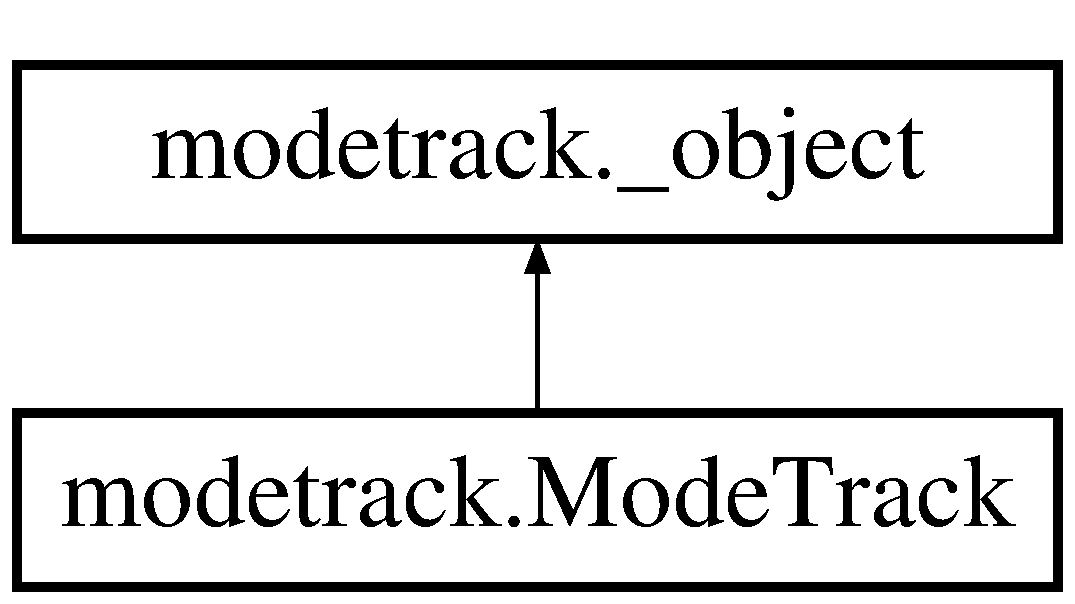
\includegraphics[height=2.000000cm]{classmodetrack_1_1_mode_track}
\end{center}
\end{figure}
\subsection*{Public Member Functions}
\begin{DoxyCompactItemize}
\item 
\hypertarget{classmodetrack_1_1_mode_track_a05a40b2371bdb331c86755f34fe85347}{def {\bfseries \-\_\-\-\_\-init\-\_\-\-\_\-}}\label{classmodetrack_1_1_mode_track_a05a40b2371bdb331c86755f34fe85347}

\item 
\hypertarget{classmodetrack_1_1_mode_track_ad7ab77246ecc717a352882bea5201f13}{def {\bfseries From\-File}}\label{classmodetrack_1_1_mode_track_ad7ab77246ecc717a352882bea5201f13}

\item 
\hypertarget{classmodetrack_1_1_mode_track_a964d6958417955c98f47d5db35b46cbe}{def {\bfseries Set\-Background}}\label{classmodetrack_1_1_mode_track_a964d6958417955c98f47d5db35b46cbe}

\item 
\hypertarget{classmodetrack_1_1_mode_track_a4c6135da338d0881912e48ad911da482}{def {\bfseries Get\-Peaks\-Gauss}}\label{classmodetrack_1_1_mode_track_a4c6135da338d0881912e48ad911da482}

\item 
\hypertarget{classmodetrack_1_1_mode_track_a0c459a1807722879287fbab923625008}{def {\bfseries Get\-Peaks\-Bi\-Lat}}\label{classmodetrack_1_1_mode_track_a0c459a1807722879287fbab923625008}

\item 
\hypertarget{classmodetrack_1_1_mode_track_a2318fd84fc3be09ba323d33f8e3cd453}{def {\bfseries Get\-Max\-Peak}}\label{classmodetrack_1_1_mode_track_a2318fd84fc3be09ba323d33f8e3cd453}

\end{DoxyCompactItemize}
\subsection*{Public Attributes}
\begin{DoxyCompactItemize}
\item 
\hypertarget{classmodetrack_1_1_mode_track_ac6b9113e1571b427ea59b3347314cee5}{{\bfseries this}}\label{classmodetrack_1_1_mode_track_ac6b9113e1571b427ea59b3347314cee5}

\end{DoxyCompactItemize}


The documentation for this class was generated from the following file\-:\begin{DoxyCompactItemize}
\item 
/home/bephillips2/workspace/\-Electric\-\_\-\-Tiger\-\_\-\-Control\-\_\-\-Code/modetrack.\-py\end{DoxyCompactItemize}

\hypertarget{classmode__tracking_1_1_mode_track_body}{\section{mode\-\_\-tracking.\-Mode\-Track\-Body Class Reference}
\label{classmode__tracking_1_1_mode_track_body}\index{mode\-\_\-tracking.\-Mode\-Track\-Body@{mode\-\_\-tracking.\-Mode\-Track\-Body}}
}
Inheritance diagram for mode\-\_\-tracking.\-Mode\-Track\-Body\-:\begin{figure}[H]
\begin{center}
\leavevmode
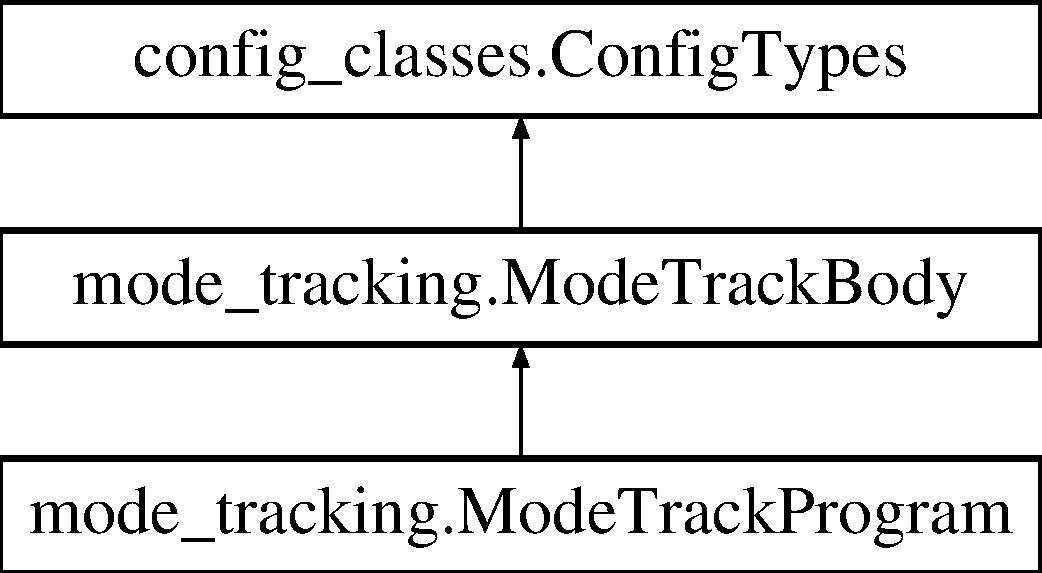
\includegraphics[height=3.000000cm]{classmode__tracking_1_1_mode_track_body}
\end{center}
\end{figure}
\subsection*{Public Member Functions}
\begin{DoxyCompactItemize}
\item 
\hypertarget{classmode__tracking_1_1_mode_track_body_ae869a3f9eb7e7e403da7358493d8fb0b}{def {\bfseries \-\_\-\-\_\-init\-\_\-\-\_\-}}\label{classmode__tracking_1_1_mode_track_body_ae869a3f9eb7e7e403da7358493d8fb0b}

\item 
\hypertarget{classmode__tracking_1_1_mode_track_body_a88caab3c24be5410d6503b93a57a6639}{def {\bfseries retract\-\_\-cavity}}\label{classmode__tracking_1_1_mode_track_body_a88caab3c24be5410d6503b93a57a6639}

\item 
\hypertarget{classmode__tracking_1_1_mode_track_body_a03b6d5d5e41558a4a83d18b6b153c23e}{def {\bfseries prequel}}\label{classmode__tracking_1_1_mode_track_body_a03b6d5d5e41558a4a83d18b6b153c23e}

\item 
\hypertarget{classmode__tracking_1_1_mode_track_body_aff9a6636f652e5f1447e7baaff664d2b}{def {\bfseries get\-\_\-data\-\_\-nwa}}\label{classmode__tracking_1_1_mode_track_body_aff9a6636f652e5f1447e7baaff664d2b}

\item 
\hypertarget{classmode__tracking_1_1_mode_track_body_a6217026364bdee7bdb38539df136d3e1}{def {\bfseries format\-\_\-points}}\label{classmode__tracking_1_1_mode_track_body_a6217026364bdee7bdb38539df136d3e1}

\item 
\hypertarget{classmode__tracking_1_1_mode_track_body_a134ec4feac3baa6fdba401314bf36569}{def {\bfseries set\-\_\-bg\-\_\-data}}\label{classmode__tracking_1_1_mode_track_body_a134ec4feac3baa6fdba401314bf36569}

\item 
\hypertarget{classmode__tracking_1_1_mode_track_body_a1ba98cc4cf92d7f6f528442da4c9bf27}{def {\bfseries find\-\_\-minima\-\_\-peak}}\label{classmode__tracking_1_1_mode_track_body_a1ba98cc4cf92d7f6f528442da4c9bf27}

\item 
\hypertarget{classmode__tracking_1_1_mode_track_body_af2c12b1611a734a5abda3b3dec54d694}{def {\bfseries next\-\_\-iteration}}\label{classmode__tracking_1_1_mode_track_body_af2c12b1611a734a5abda3b3dec54d694}

\item 
\hypertarget{classmode__tracking_1_1_mode_track_body_a7f7af78078cc7f2d44983efd5485fb1c}{def {\bfseries check\-\_\-peak}}\label{classmode__tracking_1_1_mode_track_body_a7f7af78078cc7f2d44983efd5485fb1c}

\item 
\hypertarget{classmode__tracking_1_1_mode_track_body_a65025f54e5404de32eef4947fcf94117}{def {\bfseries get\-\_\-data\-\_\-sa}}\label{classmode__tracking_1_1_mode_track_body_a65025f54e5404de32eef4947fcf94117}

\end{DoxyCompactItemize}
\subsection*{Public Attributes}
\begin{DoxyCompactItemize}
\item 
\hypertarget{classmode__tracking_1_1_mode_track_body_a31eda0c924ec92d1da33d7193471a132}{{\bfseries print\-\_\-green}}\label{classmode__tracking_1_1_mode_track_body_a31eda0c924ec92d1da33d7193471a132}

\item 
\hypertarget{classmode__tracking_1_1_mode_track_body_ae24713f7c27417815e0bf71a2538ab0f}{{\bfseries print\-\_\-purple}}\label{classmode__tracking_1_1_mode_track_body_ae24713f7c27417815e0bf71a2538ab0f}

\item 
\hypertarget{classmode__tracking_1_1_mode_track_body_a7cd938bfb18a099be142d4b697e42c00}{{\bfseries print\-\_\-blue}}\label{classmode__tracking_1_1_mode_track_body_a7cd938bfb18a099be142d4b697e42c00}

\item 
\hypertarget{classmode__tracking_1_1_mode_track_body_acb3a85b23e57c6b9ae737cf3cc07b906}{{\bfseries print\-\_\-red}}\label{classmode__tracking_1_1_mode_track_body_acb3a85b23e57c6b9ae737cf3cc07b906}

\item 
\hypertarget{classmode__tracking_1_1_mode_track_body_aaef7e806ae7a3bb09bc40197fd976b2d}{{\bfseries print\-\_\-yellow}}\label{classmode__tracking_1_1_mode_track_body_aaef7e806ae7a3bb09bc40197fd976b2d}

\item 
\hypertarget{classmode__tracking_1_1_mode_track_body_a701829ec7163923f05667f9ec7cf1ce0}{{\bfseries nwa\-\_\-comm}}\label{classmode__tracking_1_1_mode_track_body_a701829ec7163923f05667f9ec7cf1ce0}

\item 
\hypertarget{classmode__tracking_1_1_mode_track_body_af099eb879e8995405e64a67bd5bb211a}{{\bfseries sa\-\_\-comm}}\label{classmode__tracking_1_1_mode_track_body_af099eb879e8995405e64a67bd5bb211a}

\item 
\hypertarget{classmode__tracking_1_1_mode_track_body_a2a1531c1dca599ab867cc07c5b1b14cc}{{\bfseries switch\-\_\-comm}}\label{classmode__tracking_1_1_mode_track_body_a2a1531c1dca599ab867cc07c5b1b14cc}

\item 
\hypertarget{classmode__tracking_1_1_mode_track_body_a895674e243e26cb3160a5f1910faf6d0}{{\bfseries step\-\_\-comm}}\label{classmode__tracking_1_1_mode_track_body_a895674e243e26cb3160a5f1910faf6d0}

\item 
\hypertarget{classmode__tracking_1_1_mode_track_body_a0c1c68a20061990126a45dcd0cacacf1}{{\bfseries fitter}}\label{classmode__tracking_1_1_mode_track_body_a0c1c68a20061990126a45dcd0cacacf1}

\item 
\hypertarget{classmode__tracking_1_1_mode_track_body_a2b6293d7b3c3152a5453fda56e5c4468}{{\bfseries plotter}}\label{classmode__tracking_1_1_mode_track_body_a2b6293d7b3c3152a5453fda56e5c4468}

\item 
\hypertarget{classmode__tracking_1_1_mode_track_body_a0b79bad12a9a6ca3c1a831dbd1430d35}{{\bfseries m\-\_\-track}}\label{classmode__tracking_1_1_mode_track_body_a0b79bad12a9a6ca3c1a831dbd1430d35}

\item 
\hypertarget{classmode__tracking_1_1_mode_track_body_a833f18e6d84faf59ab164d44e1ddf4ff}{{\bfseries convertor}}\label{classmode__tracking_1_1_mode_track_body_a833f18e6d84faf59ab164d44e1ddf4ff}

\item 
\hypertarget{classmode__tracking_1_1_mode_track_body_a9aea71bb849de5874ae8c0f8faa25963}{{\bfseries freq\-\_\-window}}\label{classmode__tracking_1_1_mode_track_body_a9aea71bb849de5874ae8c0f8faa25963}

\item 
\hypertarget{classmode__tracking_1_1_mode_track_body_abd228f358fb6e5c2d62705caa3810c7c}{{\bfseries sa\-\_\-span}}\label{classmode__tracking_1_1_mode_track_body_abd228f358fb6e5c2d62705caa3810c7c}

\item 
\hypertarget{classmode__tracking_1_1_mode_track_body_a4c54b8f19d700e1fdb1482d9919e9c73}{{\bfseries sa\-\_\-averages}}\label{classmode__tracking_1_1_mode_track_body_a4c54b8f19d700e1fdb1482d9919e9c73}

\item 
\hypertarget{classmode__tracking_1_1_mode_track_body_aec57b5de48e988b36c06d459fcb81007}{{\bfseries fft\-\_\-length}}\label{classmode__tracking_1_1_mode_track_body_aec57b5de48e988b36c06d459fcb81007}

\item 
\hypertarget{classmode__tracking_1_1_mode_track_body_a472a17d01af9f7719b983f476a968b88}{{\bfseries nominal\-\_\-centers}}\label{classmode__tracking_1_1_mode_track_body_a472a17d01af9f7719b983f476a968b88}

\item 
\hypertarget{classmode__tracking_1_1_mode_track_body_a51f2bf12beca4a60d0954cbf5962cdd4}{{\bfseries num\-\_\-of\-\_\-iters}}\label{classmode__tracking_1_1_mode_track_body_a51f2bf12beca4a60d0954cbf5962cdd4}

\item 
\hypertarget{classmode__tracking_1_1_mode_track_body_a47888f0f588e6ccd52d077b9775f9ca6}{{\bfseries nwa\-\_\-span}}\label{classmode__tracking_1_1_mode_track_body_a47888f0f588e6ccd52d077b9775f9ca6}

\item 
\hypertarget{classmode__tracking_1_1_mode_track_body_a65be50c6c31cb99e0187d89f53f9938b}{{\bfseries fitted\-\_\-q}}\label{classmode__tracking_1_1_mode_track_body_a65be50c6c31cb99e0187d89f53f9938b}

\item 
\hypertarget{classmode__tracking_1_1_mode_track_body_a14e392077e43233fa9d9aff80a52dcde}{{\bfseries fitted\-\_\-center\-\_\-freq}}\label{classmode__tracking_1_1_mode_track_body_a14e392077e43233fa9d9aff80a52dcde}

\item 
\hypertarget{classmode__tracking_1_1_mode_track_body_ad521e295cec5960c2f3e5535bd9e66cb}{{\bfseries fitted\-\_\-height}}\label{classmode__tracking_1_1_mode_track_body_ad521e295cec5960c2f3e5535bd9e66cb}

\item 
\hypertarget{classmode__tracking_1_1_mode_track_body_a5eab268d1cd84e9735d3db2220862ed4}{{\bfseries formatted\-\_\-points}}\label{classmode__tracking_1_1_mode_track_body_a5eab268d1cd84e9735d3db2220862ed4}

\item 
\hypertarget{classmode__tracking_1_1_mode_track_body_ab4fd3beb35ac328d11f378e4fdfe7942}{{\bfseries mode\-\_\-of\-\_\-desire}}\label{classmode__tracking_1_1_mode_track_body_ab4fd3beb35ac328d11f378e4fdfe7942}

\item 
\hypertarget{classmode__tracking_1_1_mode_track_body_a03670827ec064055a8ecdb486a6cce55}{{\bfseries iteration}}\label{classmode__tracking_1_1_mode_track_body_a03670827ec064055a8ecdb486a6cce55}

\end{DoxyCompactItemize}


The documentation for this class was generated from the following file\-:\begin{DoxyCompactItemize}
\item 
/home/bephillips2/workspace/\-Electric\-\_\-\-Tiger\-\_\-\-Control\-\_\-\-Code/mode\-\_\-tracking.\-py\end{DoxyCompactItemize}

\hypertarget{classmode__tracking_1_1_mode_track_program}{\section{mode\-\_\-tracking.\-Mode\-Track\-Program Class Reference}
\label{classmode__tracking_1_1_mode_track_program}\index{mode\-\_\-tracking.\-Mode\-Track\-Program@{mode\-\_\-tracking.\-Mode\-Track\-Program}}
}
Inheritance diagram for mode\-\_\-tracking.\-Mode\-Track\-Program\-:\begin{figure}[H]
\begin{center}
\leavevmode
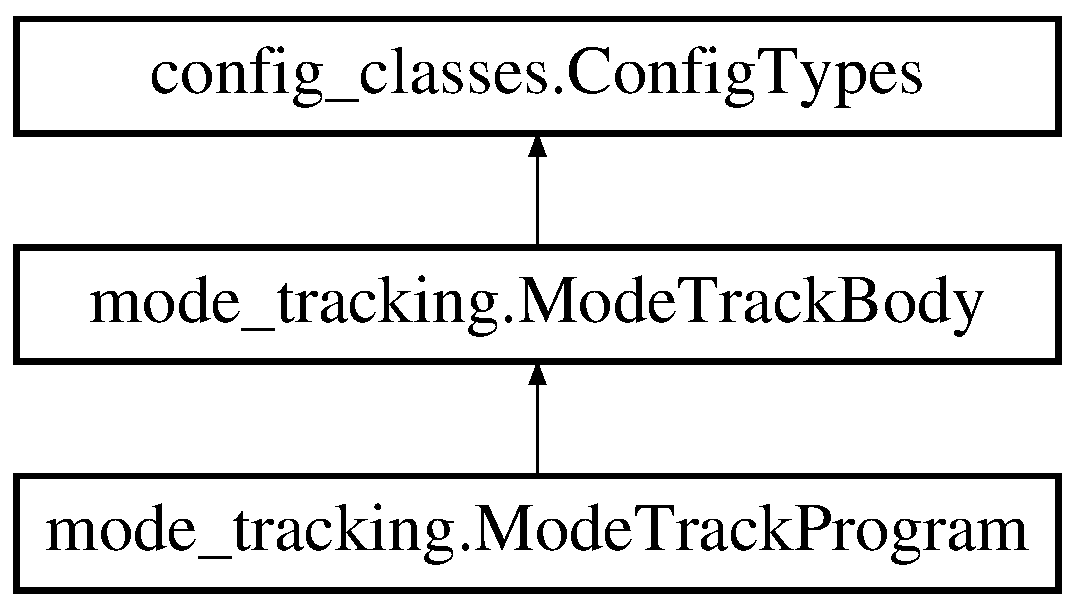
\includegraphics[height=3.000000cm]{classmode__tracking_1_1_mode_track_program}
\end{center}
\end{figure}
\subsection*{Public Member Functions}
\begin{DoxyCompactItemize}
\item 
\hypertarget{classmode__tracking_1_1_mode_track_program_afbf19a48de99b186ea59ba6fd0fa78c5}{def {\bfseries \-\_\-\-\_\-init\-\_\-\-\_\-}}\label{classmode__tracking_1_1_mode_track_program_afbf19a48de99b186ea59ba6fd0fa78c5}

\item 
\hypertarget{classmode__tracking_1_1_mode_track_program_a744015ceeefc004994908aa32cdc386e}{def {\bfseries find\-\_\-mode\-\_\-of\-\_\-desire\-\_\-reflection}}\label{classmode__tracking_1_1_mode_track_program_a744015ceeefc004994908aa32cdc386e}

\item 
\hypertarget{classmode__tracking_1_1_mode_track_program_ae35b080e6d60c56efad0719df887350c}{def {\bfseries find\-\_\-mode\-\_\-of\-\_\-desire\-\_\-transmission}}\label{classmode__tracking_1_1_mode_track_program_ae35b080e6d60c56efad0719df887350c}

\item 
\hypertarget{classmode__tracking_1_1_mode_track_program_ae4e01df4f05f30a04bfd58d8e740302e}{def {\bfseries take\-\_\-data}}\label{classmode__tracking_1_1_mode_track_program_ae4e01df4f05f30a04bfd58d8e740302e}

\item 
\hypertarget{classmode__tracking_1_1_mode_track_program_a40c65500c8890855a284cc5aeacc2f0b}{def {\bfseries set\-\_\-background}}\label{classmode__tracking_1_1_mode_track_program_a40c65500c8890855a284cc5aeacc2f0b}

\item 
\hypertarget{classmode__tracking_1_1_mode_track_program_af4cb7b240fadd3e13d72de657471203c}{def {\bfseries generate\-\_\-save\-\_\-file\-\_\-name}}\label{classmode__tracking_1_1_mode_track_program_af4cb7b240fadd3e13d72de657471203c}

\item 
\hypertarget{classmode__tracking_1_1_mode_track_program_a90da8800bc7d030f948911aef9d599c0}{def {\bfseries save\-\_\-data}}\label{classmode__tracking_1_1_mode_track_program_a90da8800bc7d030f948911aef9d599c0}

\item 
\hypertarget{classmode__tracking_1_1_mode_track_program_a2c561b201beccdd18632a0b2d0eabe72}{def {\bfseries program}}\label{classmode__tracking_1_1_mode_track_program_a2c561b201beccdd18632a0b2d0eabe72}

\item 
\hypertarget{classmode__tracking_1_1_mode_track_program_a69a58d0fdac58bc08495a9d41c5fb80d}{def {\bfseries panic\-\_\-cleanup}}\label{classmode__tracking_1_1_mode_track_program_a69a58d0fdac58bc08495a9d41c5fb80d}

\end{DoxyCompactItemize}
\subsection*{Additional Inherited Members}


The documentation for this class was generated from the following file\-:\begin{DoxyCompactItemize}
\item 
/home/bephillips2/workspace/\-Electric\-\_\-\-Tiger\-\_\-\-Control\-\_\-\-Code/mode\-\_\-tracking.\-py\end{DoxyCompactItemize}

\hypertarget{classsocket__communicators_1_1_network_analyzer_comm}{\section{socket\-\_\-communicators.\-Network\-Analyzer\-Comm Class Reference}
\label{classsocket__communicators_1_1_network_analyzer_comm}\index{socket\-\_\-communicators.\-Network\-Analyzer\-Comm@{socket\-\_\-communicators.\-Network\-Analyzer\-Comm}}
}
Inheritance diagram for socket\-\_\-communicators.\-Network\-Analyzer\-Comm\-:\begin{figure}[H]
\begin{center}
\leavevmode
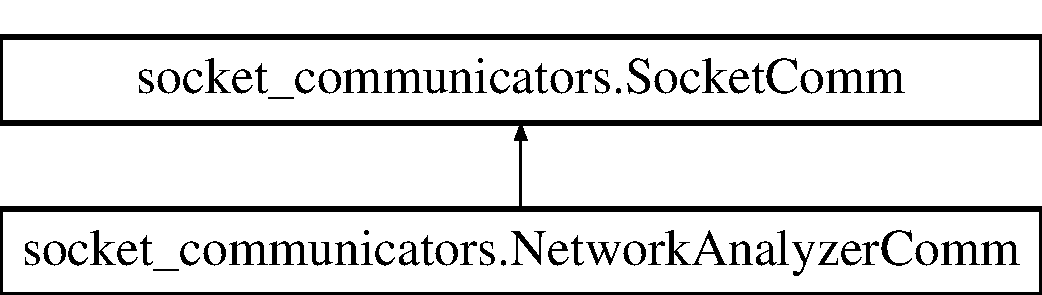
\includegraphics[height=2.000000cm]{classsocket__communicators_1_1_network_analyzer_comm}
\end{center}
\end{figure}
\subsection*{Public Member Functions}
\begin{DoxyCompactItemize}
\item 
\hypertarget{classsocket__communicators_1_1_network_analyzer_comm_a209ee51a068801999157f62644fe242d}{def {\bfseries \-\_\-\-\_\-init\-\_\-\-\_\-}}\label{classsocket__communicators_1_1_network_analyzer_comm_a209ee51a068801999157f62644fe242d}

\item 
\hypertarget{classsocket__communicators_1_1_network_analyzer_comm_a95a2c7743bb11fd9b874efa6f3d11036}{def {\bfseries collect\-\_\-data}}\label{classsocket__communicators_1_1_network_analyzer_comm_a95a2c7743bb11fd9b874efa6f3d11036}

\item 
\hypertarget{classsocket__communicators_1_1_network_analyzer_comm_a6a267091c41f5b54e87a4cd2053d1e01}{def {\bfseries set\-\_\-freq\-\_\-window}}\label{classsocket__communicators_1_1_network_analyzer_comm_a6a267091c41f5b54e87a4cd2053d1e01}

\item 
\hypertarget{classsocket__communicators_1_1_network_analyzer_comm_a3b76423b7fe0c3f4a68dafb80cf49e15}{def {\bfseries take\-\_\-data\-\_\-single}}\label{classsocket__communicators_1_1_network_analyzer_comm_a3b76423b7fe0c3f4a68dafb80cf49e15}

\end{DoxyCompactItemize}
\subsection*{Public Attributes}
\begin{DoxyCompactItemize}
\item 
\hypertarget{classsocket__communicators_1_1_network_analyzer_comm_a49e827e1462940614fef5cd5f3434bed}{{\bfseries nwa\-\_\-sock}}\label{classsocket__communicators_1_1_network_analyzer_comm_a49e827e1462940614fef5cd5f3434bed}

\end{DoxyCompactItemize}


The documentation for this class was generated from the following file\-:\begin{DoxyCompactItemize}
\item 
/home/bephillips2/workspace/\-Electric\-\_\-\-Tiger\-\_\-\-Control\-\_\-\-Code/socket\-\_\-communicators.\-py\end{DoxyCompactItemize}

\hypertarget{classdata__processors_1_1_plotter}{\section{data\-\_\-processors.\-Plotter Class Reference}
\label{classdata__processors_1_1_plotter}\index{data\-\_\-processors.\-Plotter@{data\-\_\-processors.\-Plotter}}
}
\subsection*{Public Member Functions}
\begin{DoxyCompactItemize}
\item 
\hypertarget{classdata__processors_1_1_plotter_a27acd3242a67c8140c1c99c2a1b8d9e8}{def {\bfseries \-\_\-\-\_\-call\-\_\-\-\_\-}}\label{classdata__processors_1_1_plotter_a27acd3242a67c8140c1c99c2a1b8d9e8}

\end{DoxyCompactItemize}


The documentation for this class was generated from the following file\-:\begin{DoxyCompactItemize}
\item 
/home/bephillips2/workspace/\-Electric\-\_\-\-Tiger\-\_\-\-Control\-\_\-\-Code/data\-\_\-processors.\-py\end{DoxyCompactItemize}

\hypertarget{struct_py_heap_type_object}{\section{Py\-Heap\-Type\-Object Struct Reference}
\label{struct_py_heap_type_object}\index{Py\-Heap\-Type\-Object@{Py\-Heap\-Type\-Object}}
}
\subsection*{Public Attributes}
\begin{DoxyCompactItemize}
\item 
\hypertarget{struct_py_heap_type_object_a8b961137de4ebeed5a5d2e4b47ee1ca7}{Py\-Type\-Object {\bfseries type}}\label{struct_py_heap_type_object_a8b961137de4ebeed5a5d2e4b47ee1ca7}

\item 
\hypertarget{struct_py_heap_type_object_a795de378df40d11321c0dbe463759560}{Py\-Number\-Methods {\bfseries as\-\_\-number}}\label{struct_py_heap_type_object_a795de378df40d11321c0dbe463759560}

\item 
\hypertarget{struct_py_heap_type_object_a3112d193aea288a92036360bec1ce0a5}{Py\-Mapping\-Methods {\bfseries as\-\_\-mapping}}\label{struct_py_heap_type_object_a3112d193aea288a92036360bec1ce0a5}

\item 
\hypertarget{struct_py_heap_type_object_ad553caad5da3a7004aae1b7ac0289f12}{Py\-Sequence\-Methods {\bfseries as\-\_\-sequence}}\label{struct_py_heap_type_object_ad553caad5da3a7004aae1b7ac0289f12}

\item 
\hypertarget{struct_py_heap_type_object_a026c64b0a5163ea580e79640ecf209de}{Py\-Buffer\-Procs {\bfseries as\-\_\-buffer}}\label{struct_py_heap_type_object_a026c64b0a5163ea580e79640ecf209de}

\item 
\hypertarget{struct_py_heap_type_object_a5440c0413b3c519d996119695c957c80}{Py\-Object $\ast$ {\bfseries name}}\label{struct_py_heap_type_object_a5440c0413b3c519d996119695c957c80}

\item 
\hypertarget{struct_py_heap_type_object_a15212a8f85d939b3f4b133ecda1b62e5}{Py\-Object $\ast$ {\bfseries slots}}\label{struct_py_heap_type_object_a15212a8f85d939b3f4b133ecda1b62e5}

\end{DoxyCompactItemize}


The documentation for this struct was generated from the following file\-:\begin{DoxyCompactItemize}
\item 
/home/bephillips2/workspace/\-Electric\-\_\-\-Tiger\-\_\-\-Control\-\_\-\-Code/modetrack\-\_\-wrap.\-cpp\end{DoxyCompactItemize}

\hypertarget{struct_retrieve_val}{\section{Retrieve\-Val Struct Reference}
\label{struct_retrieve_val}\index{Retrieve\-Val@{Retrieve\-Val}}
}
\subsection*{Public Member Functions}
\begin{DoxyCompactItemize}
\item 
\hypertarget{struct_retrieve_val_a497045c23da008812919a69049998b1e}{{\footnotesize template$<$typename T $>$ }\\T\-::first\-\_\-type {\bfseries operator()} (T key\-Value\-Pair) const }\label{struct_retrieve_val_a497045c23da008812919a69049998b1e}

\end{DoxyCompactItemize}


The documentation for this struct was generated from the following file\-:\begin{DoxyCompactItemize}
\item 
/home/bephillips2/workspace/\-Electric\-\_\-\-Tiger\-\_\-\-Control\-\_\-\-Code/modetrack.\-cpp\end{DoxyCompactItemize}

\hypertarget{classsocket__communicators_1_1_signal_analyzer_comm}{\section{socket\-\_\-communicators.\-Signal\-Analyzer\-Comm Class Reference}
\label{classsocket__communicators_1_1_signal_analyzer_comm}\index{socket\-\_\-communicators.\-Signal\-Analyzer\-Comm@{socket\-\_\-communicators.\-Signal\-Analyzer\-Comm}}
}
Inheritance diagram for socket\-\_\-communicators.\-Signal\-Analyzer\-Comm\-:\begin{figure}[H]
\begin{center}
\leavevmode
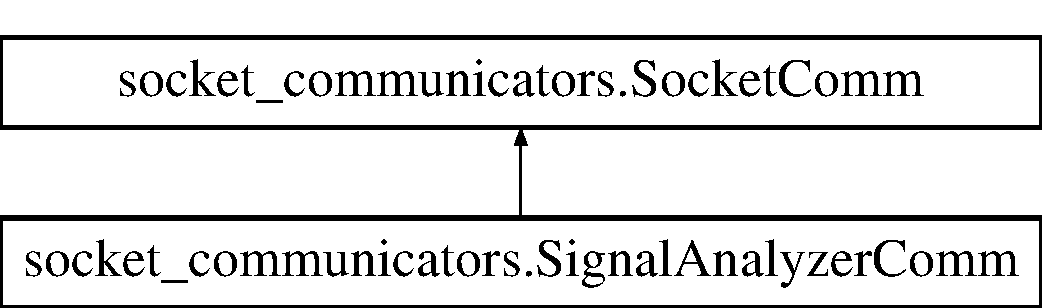
\includegraphics[height=2.000000cm]{classsocket__communicators_1_1_signal_analyzer_comm}
\end{center}
\end{figure}
\subsection*{Public Member Functions}
\begin{DoxyCompactItemize}
\item 
\hypertarget{classsocket__communicators_1_1_signal_analyzer_comm_a5e49fc639a0758b10017c0c4aeb9f905}{def {\bfseries \-\_\-\-\_\-init\-\_\-\-\_\-}}\label{classsocket__communicators_1_1_signal_analyzer_comm_a5e49fc639a0758b10017c0c4aeb9f905}

\item 
\hypertarget{classsocket__communicators_1_1_signal_analyzer_comm_a6126c357f3bed64a3504e52b79569ef2}{def {\bfseries set\-\_\-signal\-\_\-analyzer}}\label{classsocket__communicators_1_1_signal_analyzer_comm_a6126c357f3bed64a3504e52b79569ef2}

\item 
\hypertarget{classsocket__communicators_1_1_signal_analyzer_comm_a8320f6ea3a275618151f15f2416982e7}{def {\bfseries take\-\_\-data\-\_\-signal\-\_\-analyzer}}\label{classsocket__communicators_1_1_signal_analyzer_comm_a8320f6ea3a275618151f15f2416982e7}

\end{DoxyCompactItemize}
\subsection*{Public Attributes}
\begin{DoxyCompactItemize}
\item 
\hypertarget{classsocket__communicators_1_1_signal_analyzer_comm_ac389b2450afcf200f415d47659708763}{{\bfseries sa\-\_\-sock}}\label{classsocket__communicators_1_1_signal_analyzer_comm_ac389b2450afcf200f415d47659708763}

\end{DoxyCompactItemize}


The documentation for this class was generated from the following file\-:\begin{DoxyCompactItemize}
\item 
/home/bephillips2/workspace/\-Electric\-\_\-\-Tiger\-\_\-\-Control\-\_\-\-Code/socket\-\_\-communicators.\-py\end{DoxyCompactItemize}

\hypertarget{classsocket__communicators_1_1_socket_comm}{\section{socket\-\_\-communicators.\-Socket\-Comm Class Reference}
\label{classsocket__communicators_1_1_socket_comm}\index{socket\-\_\-communicators.\-Socket\-Comm@{socket\-\_\-communicators.\-Socket\-Comm}}
}
Inheritance diagram for socket\-\_\-communicators.\-Socket\-Comm\-:\begin{figure}[H]
\begin{center}
\leavevmode
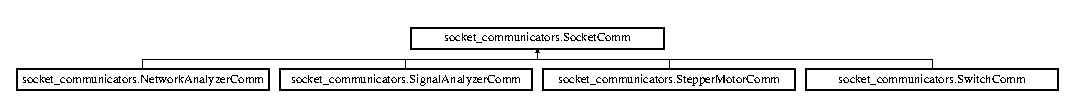
\includegraphics[height=0.992908cm]{classsocket__communicators_1_1_socket_comm}
\end{center}
\end{figure}
\subsection*{Public Member Functions}
\begin{DoxyCompactItemize}
\item 
\hypertarget{classsocket__communicators_1_1_socket_comm_aaeb5d28eb308f1b2a8f46599f60bc9d0}{def {\bfseries \-\_\-\-\_\-init\-\_\-\-\_\-}}\label{classsocket__communicators_1_1_socket_comm_aaeb5d28eb308f1b2a8f46599f60bc9d0}

\end{DoxyCompactItemize}
\subsection*{Public Attributes}
\begin{DoxyCompactItemize}
\item 
\hypertarget{classsocket__communicators_1_1_socket_comm_ab1765fc4099cff29ee2a5b254efe4d4e}{{\bfseries print\-\_\-green}}\label{classsocket__communicators_1_1_socket_comm_ab1765fc4099cff29ee2a5b254efe4d4e}

\item 
\hypertarget{classsocket__communicators_1_1_socket_comm_ad581f565c75b66877324998bbf961ae4}{{\bfseries print\-\_\-purple}}\label{classsocket__communicators_1_1_socket_comm_ad581f565c75b66877324998bbf961ae4}

\item 
\hypertarget{classsocket__communicators_1_1_socket_comm_a9d6bb220382a1a637475fce0d1dfc173}{{\bfseries print\-\_\-yellow}}\label{classsocket__communicators_1_1_socket_comm_a9d6bb220382a1a637475fce0d1dfc173}

\item 
\hypertarget{classsocket__communicators_1_1_socket_comm_a901c2955ed1807df58545e39a4952c0d}{{\bfseries print\-\_\-red}}\label{classsocket__communicators_1_1_socket_comm_a901c2955ed1807df58545e39a4952c0d}

\end{DoxyCompactItemize}


The documentation for this class was generated from the following file\-:\begin{DoxyCompactItemize}
\item 
/home/bephillips2/workspace/\-Electric\-\_\-\-Tiger\-\_\-\-Control\-\_\-\-Code/socket\-\_\-communicators.\-py\end{DoxyCompactItemize}

\hypertarget{classsocket__connect__2_1_1_socket_comm}{\section{socket\-\_\-connect\-\_\-2.\-Socket\-Comm Class Reference}
\label{classsocket__connect__2_1_1_socket_comm}\index{socket\-\_\-connect\-\_\-2.\-Socket\-Comm@{socket\-\_\-connect\-\_\-2.\-Socket\-Comm}}
}
\subsection*{Public Member Functions}
\begin{DoxyCompactItemize}
\item 
\hypertarget{classsocket__connect__2_1_1_socket_comm_a5e25404a5cede82ac3141223cb12fc7e}{def {\bfseries socket\-\_\-connect}}\label{classsocket__connect__2_1_1_socket_comm_a5e25404a5cede82ac3141223cb12fc7e}

\item 
\hypertarget{classsocket__connect__2_1_1_socket_comm_a4070a886634e0e3f6f189b19f34636b0}{def {\bfseries send\-\_\-command}}\label{classsocket__connect__2_1_1_socket_comm_a4070a886634e0e3f6f189b19f34636b0}

\item 
\hypertarget{classsocket__connect__2_1_1_socket_comm_ab7566e585f4a41553a771a03e4ba50b1}{def {\bfseries send\-\_\-command\-\_\-long}}\label{classsocket__connect__2_1_1_socket_comm_ab7566e585f4a41553a771a03e4ba50b1}

\item 
\hypertarget{classsocket__connect__2_1_1_socket_comm_afb7a59e0928bfcc49956208dc881d794}{def {\bfseries read\-\_\-data}}\label{classsocket__connect__2_1_1_socket_comm_afb7a59e0928bfcc49956208dc881d794}

\item 
\hypertarget{classsocket__connect__2_1_1_socket_comm_a2822378a14b8aa204fa97ccf177e006a}{def {\bfseries send\-\_\-command\-\_\-scl}}\label{classsocket__connect__2_1_1_socket_comm_a2822378a14b8aa204fa97ccf177e006a}

\end{DoxyCompactItemize}


The documentation for this class was generated from the following file\-:\begin{DoxyCompactItemize}
\item 
/home/bephillips2/workspace/\-Electric\-\_\-\-Tiger\-\_\-\-Control\-\_\-\-Code/socket\-\_\-connect\-\_\-2.\-py\end{DoxyCompactItemize}

\hypertarget{classsocket__communicators_1_1_stepper_motor_comm}{\section{socket\-\_\-communicators.\-Stepper\-Motor\-Comm Class Reference}
\label{classsocket__communicators_1_1_stepper_motor_comm}\index{socket\-\_\-communicators.\-Stepper\-Motor\-Comm@{socket\-\_\-communicators.\-Stepper\-Motor\-Comm}}
}
Inheritance diagram for socket\-\_\-communicators.\-Stepper\-Motor\-Comm\-:\begin{figure}[H]
\begin{center}
\leavevmode
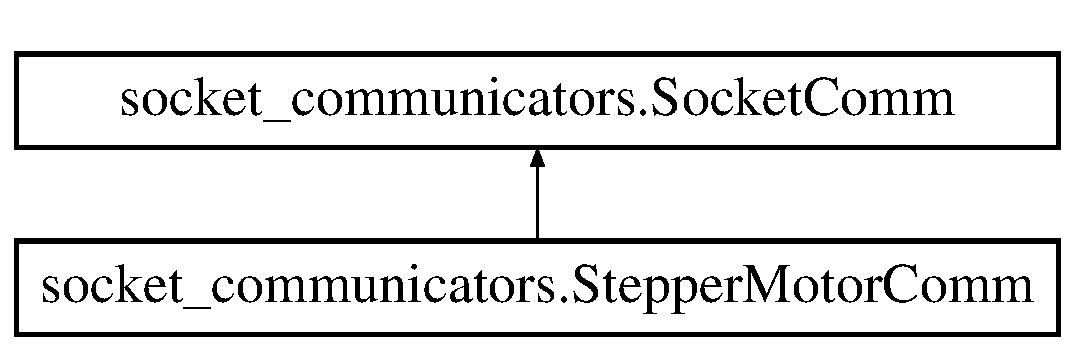
\includegraphics[height=2.000000cm]{classsocket__communicators_1_1_stepper_motor_comm}
\end{center}
\end{figure}
\subsection*{Public Member Functions}
\begin{DoxyCompactItemize}
\item 
\hypertarget{classsocket__communicators_1_1_stepper_motor_comm_ac01add7476590cc06228220173f1c6f8}{def {\bfseries \-\_\-\-\_\-init\-\_\-\-\_\-}}\label{classsocket__communicators_1_1_stepper_motor_comm_ac01add7476590cc06228220173f1c6f8}

\item 
\hypertarget{classsocket__communicators_1_1_stepper_motor_comm_a4a04ef11f6ffbf46d7a387f5ade5050f}{def {\bfseries reset\-\_\-cavity}}\label{classsocket__communicators_1_1_stepper_motor_comm_a4a04ef11f6ffbf46d7a387f5ade5050f}

\item 
\hypertarget{classsocket__communicators_1_1_stepper_motor_comm_ae81cd91ab5cb2e28dae486e6fc0301c6}{def {\bfseries panic\-\_\-reset\-\_\-cavity}}\label{classsocket__communicators_1_1_stepper_motor_comm_ae81cd91ab5cb2e28dae486e6fc0301c6}

\item 
\hypertarget{classsocket__communicators_1_1_stepper_motor_comm_ae1e0103a761a1907994f55a7663ce84a}{def {\bfseries walk\-\_\-loop}}\label{classsocket__communicators_1_1_stepper_motor_comm_ae1e0103a761a1907994f55a7663ce84a}

\end{DoxyCompactItemize}
\subsection*{Public Attributes}
\begin{DoxyCompactItemize}
\item 
\hypertarget{classsocket__communicators_1_1_stepper_motor_comm_a29f17ad6d70339459a26e3a1dcd3ed74}{{\bfseries step\-\_\-addr}}\label{classsocket__communicators_1_1_stepper_motor_comm_a29f17ad6d70339459a26e3a1dcd3ed74}

\end{DoxyCompactItemize}


The documentation for this class was generated from the following file\-:\begin{DoxyCompactItemize}
\item 
/home/bephillips2/workspace/\-Electric\-\_\-\-Tiger\-\_\-\-Control\-\_\-\-Code/socket\-\_\-communicators.\-py\end{DoxyCompactItemize}

\hypertarget{structswig__cast__info}{\section{swig\-\_\-cast\-\_\-info Struct Reference}
\label{structswig__cast__info}\index{swig\-\_\-cast\-\_\-info@{swig\-\_\-cast\-\_\-info}}
}
\subsection*{Public Attributes}
\begin{DoxyCompactItemize}
\item 
\hypertarget{structswig__cast__info_a1c9023a301c8d6806209f4e10df6e9e0}{\hyperlink{structswig__type__info}{swig\-\_\-type\-\_\-info} $\ast$ {\bfseries type}}\label{structswig__cast__info_a1c9023a301c8d6806209f4e10df6e9e0}

\item 
\hypertarget{structswig__cast__info_aa630fddfbb1bf9c97a03f9479ba32f76}{swig\-\_\-converter\-\_\-func {\bfseries converter}}\label{structswig__cast__info_aa630fddfbb1bf9c97a03f9479ba32f76}

\item 
\hypertarget{structswig__cast__info_ae79c6fa058a9d908bbdac14db0c9db5e}{struct \hyperlink{structswig__cast__info}{swig\-\_\-cast\-\_\-info} $\ast$ {\bfseries next}}\label{structswig__cast__info_ae79c6fa058a9d908bbdac14db0c9db5e}

\item 
\hypertarget{structswig__cast__info_afc685bcf38a5a06c6601775138c5999c}{struct \hyperlink{structswig__cast__info}{swig\-\_\-cast\-\_\-info} $\ast$ {\bfseries prev}}\label{structswig__cast__info_afc685bcf38a5a06c6601775138c5999c}

\end{DoxyCompactItemize}


The documentation for this struct was generated from the following file\-:\begin{DoxyCompactItemize}
\item 
/home/bephillips2/workspace/\-Electric\-\_\-\-Tiger\-\_\-\-Control\-\_\-\-Code/modetrack\-\_\-wrap.\-cpp\end{DoxyCompactItemize}

\hypertarget{structswig__const__info}{\section{swig\-\_\-const\-\_\-info Struct Reference}
\label{structswig__const__info}\index{swig\-\_\-const\-\_\-info@{swig\-\_\-const\-\_\-info}}
}
\subsection*{Public Attributes}
\begin{DoxyCompactItemize}
\item 
\hypertarget{structswig__const__info_ae8bbc99e1cda11f24e306365cbf33893}{int {\bfseries type}}\label{structswig__const__info_ae8bbc99e1cda11f24e306365cbf33893}

\item 
\hypertarget{structswig__const__info_aad383d74116313cf9a8532e163368050}{char $\ast$ {\bfseries name}}\label{structswig__const__info_aad383d74116313cf9a8532e163368050}

\item 
\hypertarget{structswig__const__info_af142e4c21ad4fe61f6c2624bff034583}{long {\bfseries lvalue}}\label{structswig__const__info_af142e4c21ad4fe61f6c2624bff034583}

\item 
\hypertarget{structswig__const__info_a74e477f1dbf515bcb7e2ef07a1d34c35}{double {\bfseries dvalue}}\label{structswig__const__info_a74e477f1dbf515bcb7e2ef07a1d34c35}

\item 
\hypertarget{structswig__const__info_abbc43512c364bff11fac5961c1155090}{void $\ast$ {\bfseries pvalue}}\label{structswig__const__info_abbc43512c364bff11fac5961c1155090}

\item 
\hypertarget{structswig__const__info_aedd46d173c5b5ed4ee60ad5660233557}{\hyperlink{structswig__type__info}{swig\-\_\-type\-\_\-info} $\ast$$\ast$ {\bfseries ptype}}\label{structswig__const__info_aedd46d173c5b5ed4ee60ad5660233557}

\end{DoxyCompactItemize}


The documentation for this struct was generated from the following file\-:\begin{DoxyCompactItemize}
\item 
/home/bephillips2/workspace/\-Electric\-\_\-\-Tiger\-\_\-\-Control\-\_\-\-Code/modetrack\-\_\-wrap.\-cpp\end{DoxyCompactItemize}

\hypertarget{structswig__globalvar}{\section{swig\-\_\-globalvar Struct Reference}
\label{structswig__globalvar}\index{swig\-\_\-globalvar@{swig\-\_\-globalvar}}
}
\subsection*{Public Attributes}
\begin{DoxyCompactItemize}
\item 
\hypertarget{structswig__globalvar_a32fcb5efb741f97e5c53e1a253cafdd9}{char $\ast$ {\bfseries name}}\label{structswig__globalvar_a32fcb5efb741f97e5c53e1a253cafdd9}

\item 
\hypertarget{structswig__globalvar_a051e346d0cd7608bf99e96726022e88c}{Py\-Object $\ast$($\ast$ {\bfseries get\-\_\-attr} )(void)}\label{structswig__globalvar_a051e346d0cd7608bf99e96726022e88c}

\item 
\hypertarget{structswig__globalvar_a494e3d5a5f1fb694b7738fdd1ffdd657}{int($\ast$ {\bfseries set\-\_\-attr} )(Py\-Object $\ast$)}\label{structswig__globalvar_a494e3d5a5f1fb694b7738fdd1ffdd657}

\item 
\hypertarget{structswig__globalvar_a6b7f8fdec3a5c39a52b33c916d7ba028}{struct \hyperlink{structswig__globalvar}{swig\-\_\-globalvar} $\ast$ {\bfseries next}}\label{structswig__globalvar_a6b7f8fdec3a5c39a52b33c916d7ba028}

\end{DoxyCompactItemize}


The documentation for this struct was generated from the following file\-:\begin{DoxyCompactItemize}
\item 
/home/bephillips2/workspace/\-Electric\-\_\-\-Tiger\-\_\-\-Control\-\_\-\-Code/modetrack\-\_\-wrap.\-cpp\end{DoxyCompactItemize}

\hypertarget{structswig__module__info}{\section{swig\-\_\-module\-\_\-info Struct Reference}
\label{structswig__module__info}\index{swig\-\_\-module\-\_\-info@{swig\-\_\-module\-\_\-info}}
}
\subsection*{Public Attributes}
\begin{DoxyCompactItemize}
\item 
\hypertarget{structswig__module__info_ad658c7738e9a035ef8eea865322fbf13}{\hyperlink{structswig__type__info}{swig\-\_\-type\-\_\-info} $\ast$$\ast$ {\bfseries types}}\label{structswig__module__info_ad658c7738e9a035ef8eea865322fbf13}

\item 
\hypertarget{structswig__module__info_aaf8907cf8509ee0464af8c9dfd909042}{size\-\_\-t {\bfseries size}}\label{structswig__module__info_aaf8907cf8509ee0464af8c9dfd909042}

\item 
\hypertarget{structswig__module__info_ac177d150b85ab77122089acf1f06d9c6}{struct \hyperlink{structswig__module__info}{swig\-\_\-module\-\_\-info} $\ast$ {\bfseries next}}\label{structswig__module__info_ac177d150b85ab77122089acf1f06d9c6}

\item 
\hypertarget{structswig__module__info_a76c7d5b0fc10371748616d0b6c815a17}{\hyperlink{structswig__type__info}{swig\-\_\-type\-\_\-info} $\ast$$\ast$ {\bfseries type\-\_\-initial}}\label{structswig__module__info_a76c7d5b0fc10371748616d0b6c815a17}

\item 
\hypertarget{structswig__module__info_a15f6b50a41f144afb1148fc412dc01f7}{\hyperlink{structswig__cast__info}{swig\-\_\-cast\-\_\-info} $\ast$$\ast$ {\bfseries cast\-\_\-initial}}\label{structswig__module__info_a15f6b50a41f144afb1148fc412dc01f7}

\item 
\hypertarget{structswig__module__info_a9fb6e461fcaf14c209049adfae4e9754}{void $\ast$ {\bfseries clientdata}}\label{structswig__module__info_a9fb6e461fcaf14c209049adfae4e9754}

\end{DoxyCompactItemize}


The documentation for this struct was generated from the following file\-:\begin{DoxyCompactItemize}
\item 
/home/bephillips2/workspace/\-Electric\-\_\-\-Tiger\-\_\-\-Control\-\_\-\-Code/modetrack\-\_\-wrap.\-cpp\end{DoxyCompactItemize}

\hypertarget{structswig__type__info}{\section{swig\-\_\-type\-\_\-info Struct Reference}
\label{structswig__type__info}\index{swig\-\_\-type\-\_\-info@{swig\-\_\-type\-\_\-info}}
}
\subsection*{Public Attributes}
\begin{DoxyCompactItemize}
\item 
\hypertarget{structswig__type__info_a90a9c6a25aa3e923978005ecbe23ad60}{const char $\ast$ {\bfseries name}}\label{structswig__type__info_a90a9c6a25aa3e923978005ecbe23ad60}

\item 
\hypertarget{structswig__type__info_abbe7cc58a083feb4329b748643324064}{const char $\ast$ {\bfseries str}}\label{structswig__type__info_abbe7cc58a083feb4329b748643324064}

\item 
\hypertarget{structswig__type__info_a07df4bedf85be77b23756b531b60e0dd}{swig\-\_\-dycast\-\_\-func {\bfseries dcast}}\label{structswig__type__info_a07df4bedf85be77b23756b531b60e0dd}

\item 
\hypertarget{structswig__type__info_a3ee3f7ef20e965b6c798d79723a96f9b}{struct \hyperlink{structswig__cast__info}{swig\-\_\-cast\-\_\-info} $\ast$ {\bfseries cast}}\label{structswig__type__info_a3ee3f7ef20e965b6c798d79723a96f9b}

\item 
\hypertarget{structswig__type__info_a19bdd65dceb89cd54befd3ded06558b7}{void $\ast$ {\bfseries clientdata}}\label{structswig__type__info_a19bdd65dceb89cd54befd3ded06558b7}

\item 
\hypertarget{structswig__type__info_a93c25d5903cbfcb82208eea7227c32bd}{int {\bfseries owndata}}\label{structswig__type__info_a93c25d5903cbfcb82208eea7227c32bd}

\end{DoxyCompactItemize}


The documentation for this struct was generated from the following file\-:\begin{DoxyCompactItemize}
\item 
/home/bephillips2/workspace/\-Electric\-\_\-\-Tiger\-\_\-\-Control\-\_\-\-Code/modetrack\-\_\-wrap.\-cpp\end{DoxyCompactItemize}

\hypertarget{structswig__varlinkobject}{\section{swig\-\_\-varlinkobject Struct Reference}
\label{structswig__varlinkobject}\index{swig\-\_\-varlinkobject@{swig\-\_\-varlinkobject}}
}
\subsection*{Public Attributes}
\begin{DoxyCompactItemize}
\item 
\hypertarget{structswig__varlinkobject_a8cf96d999cdf0b28a0e90ccb6804c9bd}{Py\-Object\-\_\-\-H\-E\-A\-D \hyperlink{structswig__globalvar}{swig\-\_\-globalvar} $\ast$ {\bfseries vars}}\label{structswig__varlinkobject_a8cf96d999cdf0b28a0e90ccb6804c9bd}

\end{DoxyCompactItemize}


The documentation for this struct was generated from the following file\-:\begin{DoxyCompactItemize}
\item 
/home/bephillips2/workspace/\-Electric\-\_\-\-Tiger\-\_\-\-Control\-\_\-\-Code/modetrack\-\_\-wrap.\-cpp\end{DoxyCompactItemize}

\hypertarget{classswig_1_1_swig_ptr___py_object}{\section{swig\-:\-:Swig\-Ptr\-\_\-\-Py\-Object Class Reference}
\label{classswig_1_1_swig_ptr___py_object}\index{swig\-::\-Swig\-Ptr\-\_\-\-Py\-Object@{swig\-::\-Swig\-Ptr\-\_\-\-Py\-Object}}
}
Inheritance diagram for swig\-:\-:Swig\-Ptr\-\_\-\-Py\-Object\-:\begin{figure}[H]
\begin{center}
\leavevmode
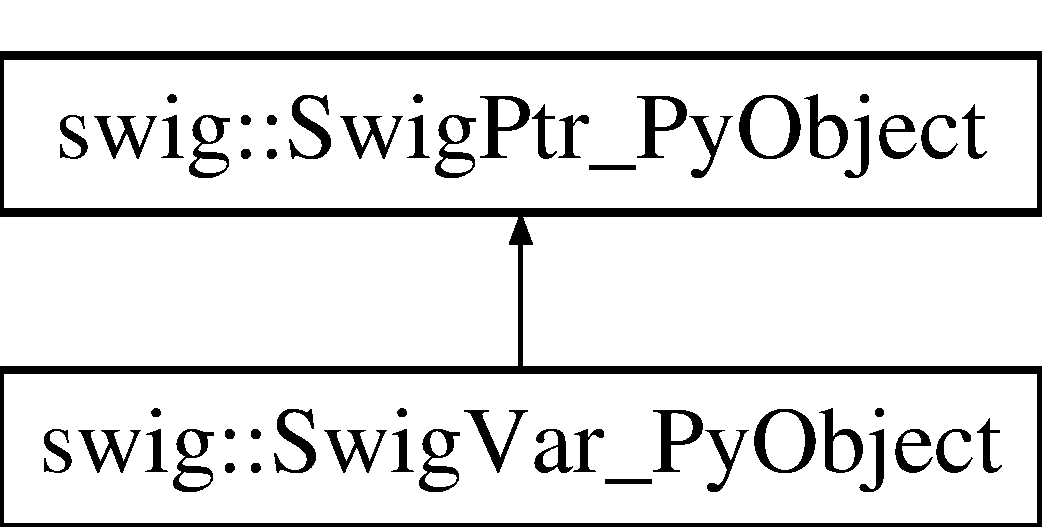
\includegraphics[height=2.000000cm]{classswig_1_1_swig_ptr___py_object}
\end{center}
\end{figure}
\subsection*{Public Member Functions}
\begin{DoxyCompactItemize}
\item 
\hypertarget{classswig_1_1_swig_ptr___py_object_a4282f20207f8cd22c9b079203c832a04}{{\bfseries Swig\-Ptr\-\_\-\-Py\-Object} (const \hyperlink{classswig_1_1_swig_ptr___py_object}{Swig\-Ptr\-\_\-\-Py\-Object} \&item)}\label{classswig_1_1_swig_ptr___py_object_a4282f20207f8cd22c9b079203c832a04}

\item 
\hypertarget{classswig_1_1_swig_ptr___py_object_a4503d58d577d209f5e1fa67026852505}{{\bfseries Swig\-Ptr\-\_\-\-Py\-Object} (Py\-Object $\ast$obj, bool initial\-\_\-ref=true)}\label{classswig_1_1_swig_ptr___py_object_a4503d58d577d209f5e1fa67026852505}

\item 
\hypertarget{classswig_1_1_swig_ptr___py_object_a86d8657d6b4a27c8e9e6942bc1ba572c}{\hyperlink{classswig_1_1_swig_ptr___py_object}{Swig\-Ptr\-\_\-\-Py\-Object} \& {\bfseries operator=} (const \hyperlink{classswig_1_1_swig_ptr___py_object}{Swig\-Ptr\-\_\-\-Py\-Object} \&item)}\label{classswig_1_1_swig_ptr___py_object_a86d8657d6b4a27c8e9e6942bc1ba572c}

\item 
\hypertarget{classswig_1_1_swig_ptr___py_object_aa2f1cdba0651c7a52482d225faef0574}{{\bfseries operator Py\-Object $\ast$} () const }\label{classswig_1_1_swig_ptr___py_object_aa2f1cdba0651c7a52482d225faef0574}

\item 
\hypertarget{classswig_1_1_swig_ptr___py_object_a97a20cad6a2b0916f39c45555fb559f0}{Py\-Object $\ast$ {\bfseries operator-\/$>$} () const }\label{classswig_1_1_swig_ptr___py_object_a97a20cad6a2b0916f39c45555fb559f0}

\end{DoxyCompactItemize}
\subsection*{Protected Attributes}
\begin{DoxyCompactItemize}
\item 
\hypertarget{classswig_1_1_swig_ptr___py_object_ae617c5726496db423cd19688e3264618}{Py\-Object $\ast$ {\bfseries \-\_\-obj}}\label{classswig_1_1_swig_ptr___py_object_ae617c5726496db423cd19688e3264618}

\end{DoxyCompactItemize}


The documentation for this class was generated from the following file\-:\begin{DoxyCompactItemize}
\item 
/home/bephillips2/workspace/\-Electric\-\_\-\-Tiger\-\_\-\-Control\-\_\-\-Code/modetrack\-\_\-wrap.\-cpp\end{DoxyCompactItemize}

\hypertarget{struct_swig_py_client_data}{\section{Swig\-Py\-Client\-Data Struct Reference}
\label{struct_swig_py_client_data}\index{Swig\-Py\-Client\-Data@{Swig\-Py\-Client\-Data}}
}
\subsection*{Public Attributes}
\begin{DoxyCompactItemize}
\item 
\hypertarget{struct_swig_py_client_data_a482d64908147c310a56d1541476079dc}{Py\-Object $\ast$ {\bfseries klass}}\label{struct_swig_py_client_data_a482d64908147c310a56d1541476079dc}

\item 
\hypertarget{struct_swig_py_client_data_a4da9e7723a1319cb42cda4ad186f65a3}{Py\-Object $\ast$ {\bfseries newraw}}\label{struct_swig_py_client_data_a4da9e7723a1319cb42cda4ad186f65a3}

\item 
\hypertarget{struct_swig_py_client_data_a8f6dacca2c445f175d622fb9264e3715}{Py\-Object $\ast$ {\bfseries newargs}}\label{struct_swig_py_client_data_a8f6dacca2c445f175d622fb9264e3715}

\item 
\hypertarget{struct_swig_py_client_data_a1c4e62712f23db599e85e24e14818d59}{Py\-Object $\ast$ {\bfseries destroy}}\label{struct_swig_py_client_data_a1c4e62712f23db599e85e24e14818d59}

\item 
\hypertarget{struct_swig_py_client_data_a9cb4b9b02743d09dbe216f304e2b7df0}{int {\bfseries delargs}}\label{struct_swig_py_client_data_a9cb4b9b02743d09dbe216f304e2b7df0}

\item 
\hypertarget{struct_swig_py_client_data_a5f9ebdbc04a774559a64b926b6ec4070}{int {\bfseries implicitconv}}\label{struct_swig_py_client_data_a5f9ebdbc04a774559a64b926b6ec4070}

\item 
\hypertarget{struct_swig_py_client_data_a1f172e51bb27f670dacdf8247843b4c2}{Py\-Type\-Object $\ast$ {\bfseries pytype}}\label{struct_swig_py_client_data_a1f172e51bb27f670dacdf8247843b4c2}

\end{DoxyCompactItemize}


The documentation for this struct was generated from the following file\-:\begin{DoxyCompactItemize}
\item 
/home/bephillips2/workspace/\-Electric\-\_\-\-Tiger\-\_\-\-Control\-\_\-\-Code/modetrack\-\_\-wrap.\-cpp\end{DoxyCompactItemize}

\hypertarget{struct_swig_py_object}{\section{Swig\-Py\-Object Struct Reference}
\label{struct_swig_py_object}\index{Swig\-Py\-Object@{Swig\-Py\-Object}}
}
\subsection*{Public Attributes}
\begin{DoxyCompactItemize}
\item 
\hypertarget{struct_swig_py_object_a41b1d569a8ba4fa9b1d87579c144891b}{Py\-Object\-\_\-\-H\-E\-A\-D void $\ast$ {\bfseries ptr}}\label{struct_swig_py_object_a41b1d569a8ba4fa9b1d87579c144891b}

\item 
\hypertarget{struct_swig_py_object_a510b5a6f66a8a33c0a54c3eeb83e5ba5}{\hyperlink{structswig__type__info}{swig\-\_\-type\-\_\-info} $\ast$ {\bfseries ty}}\label{struct_swig_py_object_a510b5a6f66a8a33c0a54c3eeb83e5ba5}

\item 
\hypertarget{struct_swig_py_object_a83cb6489fb1b171467f06c091ae6f283}{int {\bfseries own}}\label{struct_swig_py_object_a83cb6489fb1b171467f06c091ae6f283}

\item 
\hypertarget{struct_swig_py_object_af7b93d7ae49a6f3bdf6511043fe8e839}{Py\-Object $\ast$ {\bfseries next}}\label{struct_swig_py_object_af7b93d7ae49a6f3bdf6511043fe8e839}

\end{DoxyCompactItemize}


The documentation for this struct was generated from the following file\-:\begin{DoxyCompactItemize}
\item 
/home/bephillips2/workspace/\-Electric\-\_\-\-Tiger\-\_\-\-Control\-\_\-\-Code/modetrack\-\_\-wrap.\-cpp\end{DoxyCompactItemize}

\hypertarget{struct_swig_py_packed}{\section{Swig\-Py\-Packed Struct Reference}
\label{struct_swig_py_packed}\index{Swig\-Py\-Packed@{Swig\-Py\-Packed}}
}
\subsection*{Public Attributes}
\begin{DoxyCompactItemize}
\item 
\hypertarget{struct_swig_py_packed_af5122bcb9e73bf2dec4ce5f58f004e1b}{Py\-Object\-\_\-\-H\-E\-A\-D void $\ast$ {\bfseries pack}}\label{struct_swig_py_packed_af5122bcb9e73bf2dec4ce5f58f004e1b}

\item 
\hypertarget{struct_swig_py_packed_aa6f6be0a8a1bff7710200fbe8d51acf0}{\hyperlink{structswig__type__info}{swig\-\_\-type\-\_\-info} $\ast$ {\bfseries ty}}\label{struct_swig_py_packed_aa6f6be0a8a1bff7710200fbe8d51acf0}

\item 
\hypertarget{struct_swig_py_packed_aed2bfb8fb3c9f804c386215db63921cb}{size\-\_\-t {\bfseries size}}\label{struct_swig_py_packed_aed2bfb8fb3c9f804c386215db63921cb}

\end{DoxyCompactItemize}


The documentation for this struct was generated from the following file\-:\begin{DoxyCompactItemize}
\item 
/home/bephillips2/workspace/\-Electric\-\_\-\-Tiger\-\_\-\-Control\-\_\-\-Code/modetrack\-\_\-wrap.\-cpp\end{DoxyCompactItemize}

\hypertarget{structswig_1_1_swig_var___py_object}{\section{swig\-:\-:Swig\-Var\-\_\-\-Py\-Object Struct Reference}
\label{structswig_1_1_swig_var___py_object}\index{swig\-::\-Swig\-Var\-\_\-\-Py\-Object@{swig\-::\-Swig\-Var\-\_\-\-Py\-Object}}
}
Inheritance diagram for swig\-:\-:Swig\-Var\-\_\-\-Py\-Object\-:\begin{figure}[H]
\begin{center}
\leavevmode
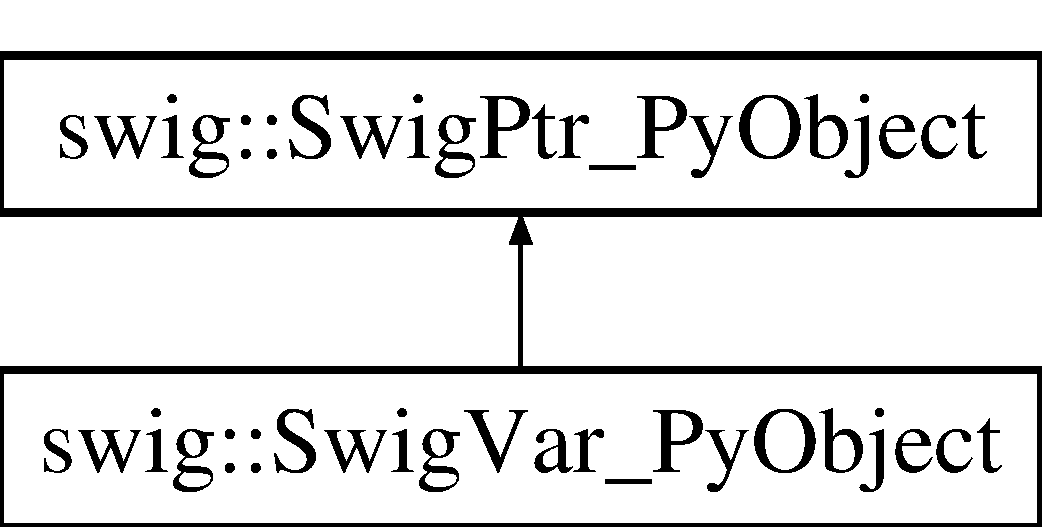
\includegraphics[height=2.000000cm]{structswig_1_1_swig_var___py_object}
\end{center}
\end{figure}
\subsection*{Public Member Functions}
\begin{DoxyCompactItemize}
\item 
\hypertarget{structswig_1_1_swig_var___py_object_a2b61f843215bceaff8ec2ea6e92d46c2}{{\bfseries Swig\-Var\-\_\-\-Py\-Object} (Py\-Object $\ast$obj=0)}\label{structswig_1_1_swig_var___py_object_a2b61f843215bceaff8ec2ea6e92d46c2}

\item 
\hypertarget{structswig_1_1_swig_var___py_object_a7e6053b64cf6e787b99a67b09cdc6d89}{\hyperlink{structswig_1_1_swig_var___py_object}{Swig\-Var\-\_\-\-Py\-Object} \& {\bfseries operator=} (Py\-Object $\ast$obj)}\label{structswig_1_1_swig_var___py_object_a7e6053b64cf6e787b99a67b09cdc6d89}

\end{DoxyCompactItemize}
\subsection*{Additional Inherited Members}


The documentation for this struct was generated from the following file\-:\begin{DoxyCompactItemize}
\item 
/home/bephillips2/workspace/\-Electric\-\_\-\-Tiger\-\_\-\-Control\-\_\-\-Code/modetrack\-\_\-wrap.\-cpp\end{DoxyCompactItemize}

\hypertarget{classsocket__communicators_1_1_switch_comm}{\section{socket\-\_\-communicators.\-Switch\-Comm Class Reference}
\label{classsocket__communicators_1_1_switch_comm}\index{socket\-\_\-communicators.\-Switch\-Comm@{socket\-\_\-communicators.\-Switch\-Comm}}
}
Inheritance diagram for socket\-\_\-communicators.\-Switch\-Comm\-:\begin{figure}[H]
\begin{center}
\leavevmode
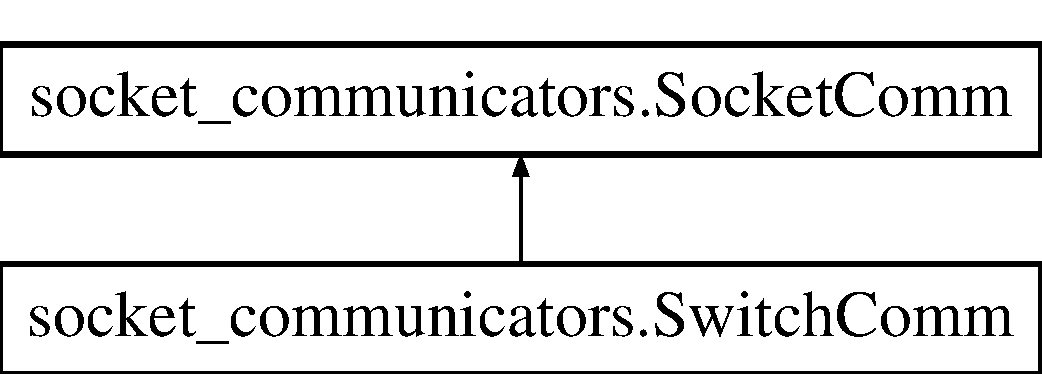
\includegraphics[height=2.000000cm]{classsocket__communicators_1_1_switch_comm}
\end{center}
\end{figure}
\subsection*{Public Member Functions}
\begin{DoxyCompactItemize}
\item 
\hypertarget{classsocket__communicators_1_1_switch_comm_adb41c0348172ce6135ce8de27218bc3e}{def {\bfseries \-\_\-\-\_\-init\-\_\-\-\_\-}}\label{classsocket__communicators_1_1_switch_comm_adb41c0348172ce6135ce8de27218bc3e}

\item 
\hypertarget{classsocket__communicators_1_1_switch_comm_a3c2f4e11a2511c8ff23da6f62128aa40}{def {\bfseries switch\-\_\-to\-\_\-signal\-\_\-analyzer}}\label{classsocket__communicators_1_1_switch_comm_a3c2f4e11a2511c8ff23da6f62128aa40}

\item 
\hypertarget{classsocket__communicators_1_1_switch_comm_a56cf447121385106dd502c138aa19fda}{def {\bfseries switch\-\_\-to\-\_\-network\-\_\-analyzer}}\label{classsocket__communicators_1_1_switch_comm_a56cf447121385106dd502c138aa19fda}

\item 
\hypertarget{classsocket__communicators_1_1_switch_comm_ab505ce5be6fc65df85a6e4134838fe4c}{def {\bfseries switch\-\_\-to\-\_\-transmission}}\label{classsocket__communicators_1_1_switch_comm_ab505ce5be6fc65df85a6e4134838fe4c}

\item 
\hypertarget{classsocket__communicators_1_1_switch_comm_a437d3ccf253331bf906c3d37f5d394ba}{def {\bfseries switch\-\_\-to\-\_\-reflection}}\label{classsocket__communicators_1_1_switch_comm_a437d3ccf253331bf906c3d37f5d394ba}

\end{DoxyCompactItemize}
\subsection*{Public Attributes}
\begin{DoxyCompactItemize}
\item 
\hypertarget{classsocket__communicators_1_1_switch_comm_abb27aeffc55e1381d52fe8f22d1d41fb}{{\bfseries switch\-\_\-sock}}\label{classsocket__communicators_1_1_switch_comm_abb27aeffc55e1381d52fe8f22d1d41fb}

\end{DoxyCompactItemize}


The documentation for this class was generated from the following file\-:\begin{DoxyCompactItemize}
\item 
/home/bephillips2/workspace/\-Electric\-\_\-\-Tiger\-\_\-\-Control\-\_\-\-Code/socket\-\_\-communicators.\-py\end{DoxyCompactItemize}

%--- End generated contents ---

% Index
\newpage
\phantomsection
\addcontentsline{toc}{chapter}{Index}
\printindex

\end{document}
